





<!DOCTYPE html>
<html lang="en">
  <head>
    <meta charset="utf-8">
  <link rel="dns-prefetch" href="https://assets-cdn.github.com">
  <link rel="dns-prefetch" href="https://avatars0.githubusercontent.com">
  <link rel="dns-prefetch" href="https://avatars1.githubusercontent.com">
  <link rel="dns-prefetch" href="https://avatars2.githubusercontent.com">
  <link rel="dns-prefetch" href="https://avatars3.githubusercontent.com">
  <link rel="dns-prefetch" href="https://github-cloud.s3.amazonaws.com">
  <link rel="dns-prefetch" href="https://user-images.githubusercontent.com/">



  <link crossorigin="anonymous" media="all" integrity="sha512-Z0JAar9+DkI1NjGVdZr3GivARUgJtA0o2eHlTv7Ou2gshR5awWVf8QGsq11Ns9ZxQLEs+G5/SuARmvpOLMzulw==" rel="stylesheet" href="https://assets-cdn.github.com/assets/frameworks-95aff0b550d3fe338b645a4deebdcb1b.css" />
  <link crossorigin="anonymous" media="all" integrity="sha512-CKx3km+/sreL8TQnawck172wM/RpBNE60XhV8wwDbn+VZlleFETFHPsSnAdaNOUySA6yFi7Xc8vX6U9P0eNhXA==" rel="stylesheet" href="https://assets-cdn.github.com/assets/github-2e6b414f4a46ee13365df9e7fbfadb35.css" />
  
  
  
  

  <meta name="viewport" content="width=device-width">
  
  <title>ActiveSubspace_Kinetics/app.tex at master · vohramanav/ActiveSubspace_Kinetics</title>
    <meta name="description" content="GitHub is where people build software. More than 28 million people use GitHub to discover, fork, and contribute to over 85 million projects.">
    <link rel="search" type="application/opensearchdescription+xml" href="/opensearch.xml" title="GitHub">
  <link rel="fluid-icon" href="https://github.com/fluidicon.png" title="GitHub">
  <meta property="fb:app_id" content="1401488693436528">

    
    <meta property="og:image" content="https://avatars1.githubusercontent.com/u/22374862?s=400&amp;v=4" /><meta property="og:site_name" content="GitHub" /><meta property="og:type" content="object" /><meta property="og:title" content="vohramanav/ActiveSubspace_Kinetics" /><meta property="og:url" content="https://github.com/vohramanav/ActiveSubspace_Kinetics" /><meta property="og:description" content="Contribute to ActiveSubspace_Kinetics development by creating an account on Github." />

  <link rel="assets" href="https://assets-cdn.github.com/">
  <link rel="web-socket" href="wss://live.github.com/_sockets/VjI6MzA5MjA1Njc0OmExZjFmODllNjEzOTRmODNiM2EzYjg2MjMxMjcwNTI2ODE5ZTg0OWE3YmRlMDYwMmRlZmZmNjFiMmMyNzI5MWY=--0d6991307d6fb87b7f9a3a145aeb29eb4bbf4bd4">
  <meta name="pjax-timeout" content="1000">
  <link rel="sudo-modal" href="/sessions/sudo_modal">
  <meta name="request-id" content="C8D0:4A98:4461DB:7F3CB3:5B7D804B" data-pjax-transient>


  

  <meta name="selected-link" value="repo_source" data-pjax-transient>

    <meta name="google-site-verification" content="KT5gs8h0wvaagLKAVWq8bbeNwnZZK1r1XQysX3xurLU">
  <meta name="google-site-verification" content="ZzhVyEFwb7w3e0-uOTltm8Jsck2F5StVihD0exw2fsA">
  <meta name="google-site-verification" content="GXs5KoUUkNCoaAZn7wPN-t01Pywp9M3sEjnt_3_ZWPc">
    <meta name="google-analytics" content="UA-3769691-2">

<meta name="octolytics-host" content="collector.githubapp.com" /><meta name="octolytics-app-id" content="github" /><meta name="octolytics-event-url" content="https://collector.githubapp.com/github-external/browser_event" /><meta name="octolytics-dimension-request_id" content="C8D0:4A98:4461DB:7F3CB3:5B7D804B" /><meta name="octolytics-dimension-region_edge" content="iad" /><meta name="octolytics-dimension-region_render" content="iad" /><meta name="octolytics-actor-id" content="22374862" /><meta name="octolytics-actor-login" content="vohramanav" /><meta name="octolytics-actor-hash" content="c3a22d3bae68f1b4588180c2c31f78aff3c5eee2ea5a5b23e0ab13a0fad0bd14" />
<meta name="analytics-location" content="/&lt;user-name&gt;/&lt;repo-name&gt;/blob/show" data-pjax-transient="true" />



  <meta class="js-ga-set" name="userId" content="d42e8fff36f702a794b24d5e9a4a8c36" %>

<meta class="js-ga-set" name="dimension1" content="Logged In">


  

      <meta name="hostname" content="github.com">
    <meta name="user-login" content="vohramanav">

      <meta name="expected-hostname" content="github.com">
    <meta name="js-proxy-site-detection-payload" content="MjU5NmUzMWQwMmNmN2RlNDU4N2Y2MGM4NjBiYTM2YTFlNGU4YzNkMDdiYWU2YzYyMzFlZjRkNDhhNTZmY2Q1OXx7InJlbW90ZV9hZGRyZXNzIjoiMTI5LjU5Ljc2LjQwIiwicmVxdWVzdF9pZCI6IkM4RDA6NEE5ODo0NDYxREI6N0YzQ0IzOjVCN0Q4MDRCIiwidGltZXN0YW1wIjoxNTM0OTUxNTAzLCJob3N0IjoiZ2l0aHViLmNvbSJ9">

    <meta name="enabled-features" content="DASHBOARD_V2_LAYOUT_OPT_IN,EXPLORE_DISCOVER_REPOSITORIES,UNIVERSE_BANNER,FREE_TRIALS,MARKETPLACE_INSIGHTS,MARKETPLACE_DOCKERFILE_CI_CTA,MARKETPLACE_PLAN_RESTRICTION_EDITOR,MARKETPLACE_SEARCH,MARKETPLACE_INSIGHTS_CONVERSION_PERCENTAGES,MARKETPLACE_RETARGETING">

  <meta name="html-safe-nonce" content="d1d04259e83798f31bc24be67464ccae1ab86a27">

  <meta http-equiv="x-pjax-version" content="6e18d0560e8611a207cfb2a7bb2a5b18">
  

      <link href="https://github.com/vohramanav/ActiveSubspace_Kinetics/commits/master.atom" rel="alternate" title="Recent Commits to ActiveSubspace_Kinetics:master" type="application/atom+xml">

  <meta name="go-import" content="github.com/vohramanav/ActiveSubspace_Kinetics git https://github.com/vohramanav/ActiveSubspace_Kinetics.git">

  <meta name="octolytics-dimension-user_id" content="22374862" /><meta name="octolytics-dimension-user_login" content="vohramanav" /><meta name="octolytics-dimension-repository_id" content="139043874" /><meta name="octolytics-dimension-repository_nwo" content="vohramanav/ActiveSubspace_Kinetics" /><meta name="octolytics-dimension-repository_public" content="true" /><meta name="octolytics-dimension-repository_is_fork" content="false" /><meta name="octolytics-dimension-repository_network_root_id" content="139043874" /><meta name="octolytics-dimension-repository_network_root_nwo" content="vohramanav/ActiveSubspace_Kinetics" /><meta name="octolytics-dimension-repository_explore_github_marketplace_ci_cta_shown" content="true" />


    <link rel="canonical" href="https://github.com/vohramanav/ActiveSubspace_Kinetics/blob/master/Paper/app.tex" data-pjax-transient>


  <meta name="browser-stats-url" content="https://api.github.com/_private/browser/stats">

  <meta name="browser-errors-url" content="https://api.github.com/_private/browser/errors">

  <link rel="mask-icon" href="https://assets-cdn.github.com/pinned-octocat.svg" color="#000000">
  <link rel="icon" type="image/x-icon" class="js-site-favicon" href="https://assets-cdn.github.com/favicon.ico">

<meta name="theme-color" content="#1e2327">



  <link rel="manifest" href="/manifest.json" crossOrigin="use-credentials">

  </head>

  <body class="logged-in env-production page-blob">
    

  <div class="position-relative js-header-wrapper ">
    <a href="#start-of-content" tabindex="1" class="p-3 bg-blue text-white show-on-focus js-skip-to-content">Skip to content</a>
    <div id="js-pjax-loader-bar" class="pjax-loader-bar"><div class="progress"></div></div>

    
    
    



        
<header class="Header  f5" role="banner">
  <div class="d-flex flex-justify-between px-3 container-lg">
    <div class="d-flex flex-justify-between ">
      <div class="">
        <a class="header-logo-invertocat" href="https://github.com/" data-hotkey="g d" aria-label="Homepage" data-ga-click="Header, go to dashboard, icon:logo">
  <svg height="32" class="octicon octicon-mark-github" viewBox="0 0 16 16" version="1.1" width="32" aria-hidden="true"><path fill-rule="evenodd" d="M8 0C3.58 0 0 3.58 0 8c0 3.54 2.29 6.53 5.47 7.59.4.07.55-.17.55-.38 0-.19-.01-.82-.01-1.49-2.01.37-2.53-.49-2.69-.94-.09-.23-.48-.94-.82-1.13-.28-.15-.68-.52-.01-.53.63-.01 1.08.58 1.23.82.72 1.21 1.87.87 2.33.66.07-.52.28-.87.51-1.07-1.78-.2-3.64-.89-3.64-3.95 0-.87.31-1.59.82-2.15-.08-.2-.36-1.02.08-2.12 0 0 .67-.21 2.2.82.64-.18 1.32-.27 2-.27.68 0 1.36.09 2 .27 1.53-1.04 2.2-.82 2.2-.82.44 1.1.16 1.92.08 2.12.51.56.82 1.27.82 2.15 0 3.07-1.87 3.75-3.65 3.95.29.25.54.73.54 1.48 0 1.07-.01 1.93-.01 2.2 0 .21.15.46.55.38A8.013 8.013 0 0 0 16 8c0-4.42-3.58-8-8-8z"/></svg>
</a>

      </div>

    </div>

    <div class="HeaderMenu d-flex flex-justify-between flex-auto">
      <div class="d-flex">
            <div class="">
              <div class="header-search scoped-search site-scoped-search js-site-search position-relative js-jump-to"
  role="search combobox"
  aria-owns="jump-to-results"
  aria-label="Search or jump to"
  aria-haspopup="listbox"
  aria-expanded="true"
>
  <div class="position-relative">
    <!-- '"` --><!-- </textarea></xmp> --></option></form><form class="js-site-search-form" data-scope-type="Repository" data-scope-id="139043874" data-scoped-search-url="/vohramanav/ActiveSubspace_Kinetics/search" data-unscoped-search-url="/search" action="/vohramanav/ActiveSubspace_Kinetics/search" accept-charset="UTF-8" method="get"><input name="utf8" type="hidden" value="&#x2713;" />
      <label class="form-control header-search-wrapper header-search-wrapper-jump-to position-relative d-flex flex-justify-between flex-items-center js-chromeless-input-container">
        <input type="text"
          class="form-control header-search-input jump-to-field js-jump-to-field js-site-search-focus js-site-search-field is-clearable"
          data-hotkey="s,/"
          name="q"
          value=""
          placeholder="Search or jump to…"
          data-unscoped-placeholder="Search or jump to…"
          data-scoped-placeholder="Search or jump to…"
          autocapitalize="off"
          aria-autocomplete="list"
          aria-controls="jump-to-results"
          data-jump-to-suggestions-path="/_graphql/GetSuggestedNavigationDestinations#csrf-token=Khu8Dh2eDlXUD2jr0BVZmOGTJeKujLMjOqtMwqFy3ShhK9UEv9eUmb6LqTqrYEPMr7se6xSia2vnRPEXKRS76A=="
          spellcheck="false"
          autocomplete="off"
          >
          <input type="hidden" class="js-site-search-type-field" name="type" >
            <img src="https://assets-cdn.github.com/images/search-shortcut-hint.svg" alt="" class="mr-2 header-search-key-slash">

            <div class="Box position-absolute overflow-hidden d-none jump-to-suggestions js-jump-to-suggestions-container">
              <ul class="d-none js-jump-to-suggestions-template-container">
                <li class="d-flex flex-justify-start flex-items-center p-0 f5 navigation-item js-navigation-item">
                  <a tabindex="-1" class="no-underline d-flex flex-auto flex-items-center p-2 jump-to-suggestions-path js-jump-to-suggestion-path js-navigation-open" href="">
                    <div class="jump-to-octicon js-jump-to-octicon mr-2 text-center d-none"></div>
                    <img class="avatar mr-2 flex-shrink-0 js-jump-to-suggestion-avatar" alt="" aria-label="Team" src="" width="28" height="28">

                    <div class="jump-to-suggestion-name js-jump-to-suggestion-name flex-auto overflow-hidden text-left no-wrap css-truncate css-truncate-target">
                    </div>

                    <div class="border rounded-1 flex-shrink-0 bg-gray px-1 text-gray-light ml-1 f6 d-none js-jump-to-badge-search">
                      <span class="js-jump-to-badge-search-text-default d-none" aria-label="in this repository">
                        In this repository
                      </span>
                      <span class="js-jump-to-badge-search-text-global d-none" aria-label="in all of GitHub">
                        All GitHub
                      </span>
                      <span aria-hidden="true" class="d-inline-block ml-1 v-align-middle">↵</span>
                    </div>

                    <div aria-hidden="true" class="border rounded-1 flex-shrink-0 bg-gray px-1 text-gray-light ml-1 f6 d-none d-on-nav-focus js-jump-to-badge-jump">
                      Jump to
                      <span class="d-inline-block ml-1 v-align-middle">↵</span>
                    </div>
                  </a>
                </li>
                <svg height="16" width="16" class="octicon octicon-repo flex-shrink-0 js-jump-to-repo-octicon-template" title="Repository" aria-label="Repository" viewBox="0 0 12 16" version="1.1" role="img"><path fill-rule="evenodd" d="M4 9H3V8h1v1zm0-3H3v1h1V6zm0-2H3v1h1V4zm0-2H3v1h1V2zm8-1v12c0 .55-.45 1-1 1H6v2l-1.5-1.5L3 16v-2H1c-.55 0-1-.45-1-1V1c0-.55.45-1 1-1h10c.55 0 1 .45 1 1zm-1 10H1v2h2v-1h3v1h5v-2zm0-10H2v9h9V1z"/></svg>
                <svg height="16" width="16" class="octicon octicon-project flex-shrink-0 js-jump-to-project-octicon-template" title="Project" aria-label="Project" viewBox="0 0 15 16" version="1.1" role="img"><path fill-rule="evenodd" d="M10 12h3V2h-3v10zm-4-2h3V2H6v8zm-4 4h3V2H2v12zm-1 1h13V1H1v14zM14 0H1a1 1 0 0 0-1 1v14a1 1 0 0 0 1 1h13a1 1 0 0 0 1-1V1a1 1 0 0 0-1-1z"/></svg>
                <svg height="16" width="16" class="octicon octicon-search flex-shrink-0 js-jump-to-search-octicon-template" title="Search" aria-label="Search" viewBox="0 0 16 16" version="1.1" role="img"><path fill-rule="evenodd" d="M15.7 13.3l-3.81-3.83A5.93 5.93 0 0 0 13 6c0-3.31-2.69-6-6-6S1 2.69 1 6s2.69 6 6 6c1.3 0 2.48-.41 3.47-1.11l3.83 3.81c.19.2.45.3.7.3.25 0 .52-.09.7-.3a.996.996 0 0 0 0-1.41v.01zM7 10.7c-2.59 0-4.7-2.11-4.7-4.7 0-2.59 2.11-4.7 4.7-4.7 2.59 0 4.7 2.11 4.7 4.7 0 2.59-2.11 4.7-4.7 4.7z"/></svg>
              </ul>
              <ul class="d-none js-jump-to-no-results-template-container">
                <li class="d-flex flex-justify-center flex-items-center p-3 f5 d-none">
                  <span class="text-gray">No suggested jump to results</span>
                </li>
              </ul>

              <ul id="jump-to-results" class="js-navigation-container jump-to-suggestions-results-container js-jump-to-suggestions-results-container" >
                <li class="d-flex flex-justify-center flex-items-center p-0 f5">
                  <img src="https://assets-cdn.github.com/images/spinners/octocat-spinner-128.gif" alt="Octocat Spinner Icon" class="m-2" width="28">
                </li>
              </ul>
            </div>
      </label>
</form>  </div>
</div>

            </div>

          <ul class="d-flex pl-2 flex-items-center text-bold list-style-none" role="navigation">
            <li>
              <a class="js-selected-navigation-item HeaderNavlink px-2" data-hotkey="g p" data-ga-click="Header, click, Nav menu - item:pulls context:user" aria-label="Pull requests you created" data-selected-links="/pulls /pulls/assigned /pulls/mentioned /pulls" href="/pulls">
                Pull requests
</a>            </li>
            <li>
              <a class="js-selected-navigation-item HeaderNavlink px-2" data-hotkey="g i" data-ga-click="Header, click, Nav menu - item:issues context:user" aria-label="Issues you created" data-selected-links="/issues /issues/assigned /issues/mentioned /issues" href="/issues">
                Issues
</a>            </li>
              <li>
                <a class="js-selected-navigation-item HeaderNavlink px-2" data-ga-click="Header, click, Nav menu - item:marketplace context:user" data-octo-click="marketplace_click" data-octo-dimensions="location:nav_bar" data-selected-links=" /marketplace" href="/marketplace">
                   Marketplace
</a>              </li>
            <li>
              <a class="js-selected-navigation-item HeaderNavlink px-2" data-ga-click="Header, click, Nav menu - item:explore" data-selected-links="/explore /trending /trending/developers /integrations /integrations/feature/code /integrations/feature/collaborate /integrations/feature/ship showcases showcases_search showcases_landing /explore" href="/explore">
                Explore
</a>            </li>
          </ul>
      </div>

      <div class="d-flex">
        
<ul class="user-nav d-flex flex-items-center list-style-none" id="user-links">
  <li class="dropdown">
    <span class="d-inline-block  px-2">
      

    </span>
  </li>

  <li class="dropdown">
    <details class="details-overlay details-reset d-flex px-2 flex-items-center">
      <summary class="HeaderNavlink"
         aria-label="Create new…"
         data-ga-click="Header, create new, icon:add">
        <svg class="octicon octicon-plus float-left mr-1 mt-1" viewBox="0 0 12 16" version="1.1" width="12" height="16" aria-hidden="true"><path fill-rule="evenodd" d="M12 9H7v5H5V9H0V7h5V2h2v5h5v2z"/></svg>
        <span class="dropdown-caret mt-1"></span>
      </summary>
      <details-menu class="dropdown-menu dropdown-menu-sw">
        
<a role="menuitem" class="dropdown-item" href="/new" data-ga-click="Header, create new repository">
  New repository
</a>

  <a role="menuitem" class="dropdown-item" href="/new/import" data-ga-click="Header, import a repository">
    Import repository
  </a>

<a role="menuitem" class="dropdown-item" href="https://gist.github.com/" data-ga-click="Header, create new gist">
  New gist
</a>

  <a role="menuitem" class="dropdown-item" href="/organizations/new" data-ga-click="Header, create new organization">
    New organization
  </a>


  <div class="dropdown-divider"></div>
  <div class="dropdown-header">
    <span title="vohramanav/ActiveSubspace_Kinetics">This repository</span>
  </div>
    <a role="menuitem" class="dropdown-item" href="/vohramanav/ActiveSubspace_Kinetics/issues/new" data-ga-click="Header, create new issue">
      New issue
    </a>

      </details-menu>
    </details>
  </li>

  <li class="dropdown">

    <details class="details-overlay details-reset d-flex pl-2 flex-items-center">
      <summary class="HeaderNavlink name mt-1"
        aria-label="View profile and more"
        data-ga-click="Header, show menu, icon:avatar">
        <img alt="@vohramanav" class="avatar float-left mr-1" src="https://avatars2.githubusercontent.com/u/22374862?s=40&amp;v=4" height="20" width="20">
        <span class="dropdown-caret"></span>
      </summary>
      <details-menu class="dropdown-menu dropdown-menu-sw">
        <ul>
          <li class="header-nav-current-user css-truncate"><a role="menuitem" class="no-underline user-profile-link px-3 pt-2 pb-2 mb-n2 mt-n1 d-block" href="/vohramanav" data-ga-click="Header, go to profile, text:Signed in as">Signed in as <strong class="css-truncate-target">vohramanav</strong></a></li>
          <li class="dropdown-divider"></li>
          <li><a role="menuitem" class="dropdown-item" href="/vohramanav" data-ga-click="Header, go to profile, text:your profile">Your profile</a></li>
          <li><a role="menuitem" class="dropdown-item" href="/vohramanav?tab=repositories" data-ga-click="Header, go to repositories, text:your repositories">Your repositories</a></li>
          <li><a role="menuitem" class="dropdown-item" href="/vohramanav?tab=stars" data-ga-click="Header, go to starred repos, text:your stars">Your stars</a></li>
            <li><a role="menuitem" class="dropdown-item" href="https://gist.github.com/" data-ga-click="Header, your gists, text:your gists">Your gists</a></li>
          <li class="dropdown-divider"></li>
          <li><a role="menuitem" class="dropdown-item" href="https://help.github.com" data-ga-click="Header, go to help, text:help">Help</a></li>
          <li><a role="menuitem" class="dropdown-item" href="/settings/profile" data-ga-click="Header, go to settings, icon:settings">Settings</a></li>
          <li>
            <!-- '"` --><!-- </textarea></xmp> --></option></form><form class="logout-form" action="/logout" accept-charset="UTF-8" method="post"><input name="utf8" type="hidden" value="&#x2713;" /><input type="hidden" name="authenticity_token" value="3FaIm4CNM+9PIkyx5NRmLAxirPlwSyU57JNLpTDpqd2yz8pM/zAEZMKa+Utzum5LjQrgvK9fti0XWce6BUIaTw==" />
              <button type="submit" class="dropdown-item dropdown-signout" data-ga-click="Header, sign out, icon:logout" role="menuitem">
                Sign out
              </button>
</form>          </li>
        </ul>
      </details-menu>
    </details>
  </li>
</ul>



        <!-- '"` --><!-- </textarea></xmp> --></option></form><form class="sr-only right-0" action="/logout" accept-charset="UTF-8" method="post"><input name="utf8" type="hidden" value="&#x2713;" /><input type="hidden" name="authenticity_token" value="sdl7U6uC/YnIEBDe0m1Ffqw8ZpCWgyX9StrMRnOb1xTfQDmE1D/KAkWopSRFA00ZLVQq1UmXtumxEEBZRjBkhg==" />
          <button type="submit" class="dropdown-item dropdown-signout" data-ga-click="Header, sign out, icon:logout">
            Sign out
          </button>
</form>      </div>
    </div>
  </div>
</header>

      

  </div>

  <div id="start-of-content" class="show-on-focus"></div>

    <div id="js-flash-container">


</div>



  <div role="main" class="application-main ">
        <div itemscope itemtype="http://schema.org/SoftwareSourceCode" class="">
    <div id="js-repo-pjax-container" data-pjax-container >
      







  <div class="pagehead repohead instapaper_ignore readability-menu experiment-repo-nav  ">
    <div class="repohead-details-container clearfix container">

      <ul class="pagehead-actions">
  <li>
        <!-- '"` --><!-- </textarea></xmp> --></option></form><form data-autosubmit="true" data-remote="true" class="js-social-container" action="/notifications/subscribe" accept-charset="UTF-8" method="post"><input name="utf8" type="hidden" value="&#x2713;" /><input type="hidden" name="authenticity_token" value="hJC2MQ3NdavI/Csfx3TSs4s2QA4FpmgBs4G2/t++I+CnF84lI3fOU89Q7x8ng6qvvNfpBemZdOJN+oksI+YsXg==" />      <input type="hidden" name="repository_id" id="repository_id" value="139043874" class="form-control" />

        <div class="select-menu js-menu-container js-select-menu">
          <a href="/vohramanav/ActiveSubspace_Kinetics/subscription"
            class="btn btn-sm btn-with-count select-menu-button js-menu-target"
            role="button"
            aria-haspopup="true"
            aria-expanded="false"
            aria-label="Toggle repository notifications menu"
            data-ga-click="Repository, click Watch settings, action:blob#show">
            <span class="js-select-button">
                <svg class="octicon octicon-eye v-align-text-bottom" viewBox="0 0 16 16" version="1.1" width="16" height="16" aria-hidden="true"><path fill-rule="evenodd" d="M8.06 2C3 2 0 8 0 8s3 6 8.06 6C13 14 16 8 16 8s-3-6-7.94-6zM8 12c-2.2 0-4-1.78-4-4 0-2.2 1.8-4 4-4 2.22 0 4 1.8 4 4 0 2.22-1.78 4-4 4zm2-4c0 1.11-.89 2-2 2-1.11 0-2-.89-2-2 0-1.11.89-2 2-2 1.11 0 2 .89 2 2z"/></svg>
                Watch
            </span>
          </a>
          <a class="social-count js-social-count"
            href="/vohramanav/ActiveSubspace_Kinetics/watchers"
            aria-label="1 user is watching this repository">
            1
          </a>

        <div class="select-menu-modal-holder">
          <div class="select-menu-modal subscription-menu-modal js-menu-content">
            <div class="select-menu-header js-navigation-enable" tabindex="-1">
              <svg class="octicon octicon-x js-menu-close" role="img" aria-label="Close" viewBox="0 0 12 16" version="1.1" width="12" height="16"><path fill-rule="evenodd" d="M7.48 8l3.75 3.75-1.48 1.48L6 9.48l-3.75 3.75-1.48-1.48L4.52 8 .77 4.25l1.48-1.48L6 6.52l3.75-3.75 1.48 1.48L7.48 8z"/></svg>
              <span class="select-menu-title">Notifications</span>
            </div>

              <div class="select-menu-list js-navigation-container" role="menu">

                <div class="select-menu-item js-navigation-item selected" role="menuitem" tabindex="0">
                  <svg class="octicon octicon-check select-menu-item-icon" viewBox="0 0 12 16" version="1.1" width="12" height="16" aria-hidden="true"><path fill-rule="evenodd" d="M12 5l-8 8-4-4 1.5-1.5L4 10l6.5-6.5L12 5z"/></svg>
                  <div class="select-menu-item-text">
                    <input type="radio" name="do" id="do_included" value="included" checked="checked" />
                    <span class="select-menu-item-heading">Not watching</span>
                    <span class="description">Be notified when participating or @mentioned.</span>
                    <span class="js-select-button-text hidden-select-button-text">
                      <svg class="octicon octicon-eye v-align-text-bottom" viewBox="0 0 16 16" version="1.1" width="16" height="16" aria-hidden="true"><path fill-rule="evenodd" d="M8.06 2C3 2 0 8 0 8s3 6 8.06 6C13 14 16 8 16 8s-3-6-7.94-6zM8 12c-2.2 0-4-1.78-4-4 0-2.2 1.8-4 4-4 2.22 0 4 1.8 4 4 0 2.22-1.78 4-4 4zm2-4c0 1.11-.89 2-2 2-1.11 0-2-.89-2-2 0-1.11.89-2 2-2 1.11 0 2 .89 2 2z"/></svg>
                      Watch
                    </span>
                  </div>
                </div>

                <div class="select-menu-item js-navigation-item " role="menuitem" tabindex="0">
                  <svg class="octicon octicon-check select-menu-item-icon" viewBox="0 0 12 16" version="1.1" width="12" height="16" aria-hidden="true"><path fill-rule="evenodd" d="M12 5l-8 8-4-4 1.5-1.5L4 10l6.5-6.5L12 5z"/></svg>
                  <div class="select-menu-item-text">
                    <input type="radio" name="do" id="do_subscribed" value="subscribed" />
                    <span class="select-menu-item-heading">Watching</span>
                    <span class="description">Be notified of all conversations.</span>
                    <span class="js-select-button-text hidden-select-button-text">
                      <svg class="octicon octicon-eye v-align-text-bottom" viewBox="0 0 16 16" version="1.1" width="16" height="16" aria-hidden="true"><path fill-rule="evenodd" d="M8.06 2C3 2 0 8 0 8s3 6 8.06 6C13 14 16 8 16 8s-3-6-7.94-6zM8 12c-2.2 0-4-1.78-4-4 0-2.2 1.8-4 4-4 2.22 0 4 1.8 4 4 0 2.22-1.78 4-4 4zm2-4c0 1.11-.89 2-2 2-1.11 0-2-.89-2-2 0-1.11.89-2 2-2 1.11 0 2 .89 2 2z"/></svg>
                        Unwatch
                    </span>
                  </div>
                </div>

                <div class="select-menu-item js-navigation-item " role="menuitem" tabindex="0">
                  <svg class="octicon octicon-check select-menu-item-icon" viewBox="0 0 12 16" version="1.1" width="12" height="16" aria-hidden="true"><path fill-rule="evenodd" d="M12 5l-8 8-4-4 1.5-1.5L4 10l6.5-6.5L12 5z"/></svg>
                  <div class="select-menu-item-text">
                    <input type="radio" name="do" id="do_ignore" value="ignore" />
                    <span class="select-menu-item-heading">Ignoring</span>
                    <span class="description">Never be notified.</span>
                    <span class="js-select-button-text hidden-select-button-text">
                      <svg class="octicon octicon-mute v-align-text-bottom" viewBox="0 0 16 16" version="1.1" width="16" height="16" aria-hidden="true"><path fill-rule="evenodd" d="M8 2.81v10.38c0 .67-.81 1-1.28.53L3 10H1c-.55 0-1-.45-1-1V7c0-.55.45-1 1-1h2l3.72-3.72C7.19 1.81 8 2.14 8 2.81zm7.53 3.22l-1.06-1.06-1.97 1.97-1.97-1.97-1.06 1.06L11.44 8 9.47 9.97l1.06 1.06 1.97-1.97 1.97 1.97 1.06-1.06L13.56 8l1.97-1.97z"/></svg>
                        Stop ignoring
                    </span>
                  </div>
                </div>

              </div>

            </div>
          </div>
        </div>
</form>
  </li>

  <li>
    
  <div class="js-toggler-container js-social-container starring-container ">
    <!-- '"` --><!-- </textarea></xmp> --></option></form><form class="starred js-social-form" action="/vohramanav/ActiveSubspace_Kinetics/unstar" accept-charset="UTF-8" method="post"><input name="utf8" type="hidden" value="&#x2713;" /><input type="hidden" name="authenticity_token" value="nlQEgDZqIDarSTmYWZRyabcRQTOKN2kHMJDtdWpsDFkcvUvB9w+isACt0PdhXndQeYd1o5R4xxsREC3j4rQGrw==" />
      <input type="hidden" name="context" value="repository"></input>
      <button
        type="submit"
        class="btn btn-sm btn-with-count js-toggler-target"
        aria-label="Unstar this repository" title="Unstar vohramanav/ActiveSubspace_Kinetics"
        data-ga-click="Repository, click unstar button, action:blob#show; text:Unstar">
        <svg class="octicon octicon-star v-align-text-bottom" viewBox="0 0 14 16" version="1.1" width="14" height="16" aria-hidden="true"><path fill-rule="evenodd" d="M14 6l-4.9-.64L7 1 4.9 5.36 0 6l3.6 3.26L2.67 14 7 11.67 11.33 14l-.93-4.74L14 6z"/></svg>
        Unstar
      </button>
        <a class="social-count js-social-count" href="/vohramanav/ActiveSubspace_Kinetics/stargazers"
           aria-label="0 users starred this repository">
          0
        </a>
</form>
    <!-- '"` --><!-- </textarea></xmp> --></option></form><form class="unstarred js-social-form" action="/vohramanav/ActiveSubspace_Kinetics/star" accept-charset="UTF-8" method="post"><input name="utf8" type="hidden" value="&#x2713;" /><input type="hidden" name="authenticity_token" value="c/RaxS+3o1dBydJ8SDGs6EgAoUEG/xq+9x5RUNJiDAmxQi21ayI25gQHGus4d0L2Jr/jPRTN7nvkgq+EYI9HdA==" />
      <input type="hidden" name="context" value="repository"></input>
      <button
        type="submit"
        class="btn btn-sm btn-with-count js-toggler-target"
        aria-label="Star this repository" title="Star vohramanav/ActiveSubspace_Kinetics"
        data-ga-click="Repository, click star button, action:blob#show; text:Star">
        <svg class="octicon octicon-star v-align-text-bottom" viewBox="0 0 14 16" version="1.1" width="14" height="16" aria-hidden="true"><path fill-rule="evenodd" d="M14 6l-4.9-.64L7 1 4.9 5.36 0 6l3.6 3.26L2.67 14 7 11.67 11.33 14l-.93-4.74L14 6z"/></svg>
        Star
      </button>
        <a class="social-count js-social-count" href="/vohramanav/ActiveSubspace_Kinetics/stargazers"
           aria-label="0 users starred this repository">
          0
        </a>
</form>  </div>

  </li>

  <li>
        <span class="btn btn-sm btn-with-count disabled tooltipped tooltipped-sw" aria-label="Cannot fork because you own this repository and are not a member of any organizations.">
          <svg class="octicon octicon-repo-forked v-align-text-bottom" viewBox="0 0 10 16" version="1.1" width="10" height="16" aria-hidden="true"><path fill-rule="evenodd" d="M8 1a1.993 1.993 0 0 0-1 3.72V6L5 8 3 6V4.72A1.993 1.993 0 0 0 2 1a1.993 1.993 0 0 0-1 3.72V6.5l3 3v1.78A1.993 1.993 0 0 0 5 15a1.993 1.993 0 0 0 1-3.72V9.5l3-3V4.72A1.993 1.993 0 0 0 8 1zM2 4.2C1.34 4.2.8 3.65.8 3c0-.65.55-1.2 1.2-1.2.65 0 1.2.55 1.2 1.2 0 .65-.55 1.2-1.2 1.2zm3 10c-.66 0-1.2-.55-1.2-1.2 0-.65.55-1.2 1.2-1.2.65 0 1.2.55 1.2 1.2 0 .65-.55 1.2-1.2 1.2zm3-10c-.66 0-1.2-.55-1.2-1.2 0-.65.55-1.2 1.2-1.2.65 0 1.2.55 1.2 1.2 0 .65-.55 1.2-1.2 1.2z"/></svg>
          Fork
</span>
    <a href="/vohramanav/ActiveSubspace_Kinetics/network/members" class="social-count"
       aria-label="0 users forked this repository">
      0
    </a>
  </li>
</ul>

      <h1 class="public ">
  <svg class="octicon octicon-repo" viewBox="0 0 12 16" version="1.1" width="12" height="16" aria-hidden="true"><path fill-rule="evenodd" d="M4 9H3V8h1v1zm0-3H3v1h1V6zm0-2H3v1h1V4zm0-2H3v1h1V2zm8-1v12c0 .55-.45 1-1 1H6v2l-1.5-1.5L3 16v-2H1c-.55 0-1-.45-1-1V1c0-.55.45-1 1-1h10c.55 0 1 .45 1 1zm-1 10H1v2h2v-1h3v1h5v-2zm0-10H2v9h9V1z"/></svg>
  <span class="author" itemprop="author"><a class="url fn" rel="author" href="/vohramanav">vohramanav</a></span><!--
--><span class="path-divider">/</span><!--
--><strong itemprop="name"><a data-pjax="#js-repo-pjax-container" href="/vohramanav/ActiveSubspace_Kinetics">ActiveSubspace_Kinetics</a></strong>

</h1>

    </div>
    
<nav class="reponav js-repo-nav js-sidenav-container-pjax container"
     itemscope
     itemtype="http://schema.org/BreadcrumbList"
     role="navigation"
     data-pjax="#js-repo-pjax-container">

  <span itemscope itemtype="http://schema.org/ListItem" itemprop="itemListElement">
    <a class="js-selected-navigation-item selected reponav-item" itemprop="url" data-hotkey="g c" data-selected-links="repo_source repo_downloads repo_commits repo_releases repo_tags repo_branches repo_packages /vohramanav/ActiveSubspace_Kinetics" href="/vohramanav/ActiveSubspace_Kinetics">
      <svg class="octicon octicon-code" viewBox="0 0 14 16" version="1.1" width="14" height="16" aria-hidden="true"><path fill-rule="evenodd" d="M9.5 3L8 4.5 11.5 8 8 11.5 9.5 13 14 8 9.5 3zm-5 0L0 8l4.5 5L6 11.5 2.5 8 6 4.5 4.5 3z"/></svg>
      <span itemprop="name">Code</span>
      <meta itemprop="position" content="1">
</a>  </span>

    <span itemscope itemtype="http://schema.org/ListItem" itemprop="itemListElement">
      <a itemprop="url" data-hotkey="g i" class="js-selected-navigation-item reponav-item" data-selected-links="repo_issues repo_labels repo_milestones /vohramanav/ActiveSubspace_Kinetics/issues" href="/vohramanav/ActiveSubspace_Kinetics/issues">
        <svg class="octicon octicon-issue-opened" viewBox="0 0 14 16" version="1.1" width="14" height="16" aria-hidden="true"><path fill-rule="evenodd" d="M7 2.3c3.14 0 5.7 2.56 5.7 5.7s-2.56 5.7-5.7 5.7A5.71 5.71 0 0 1 1.3 8c0-3.14 2.56-5.7 5.7-5.7zM7 1C3.14 1 0 4.14 0 8s3.14 7 7 7 7-3.14 7-7-3.14-7-7-7zm1 3H6v5h2V4zm0 6H6v2h2v-2z"/></svg>
        <span itemprop="name">Issues</span>
        <span class="Counter">0</span>
        <meta itemprop="position" content="2">
</a>    </span>

  <span itemscope itemtype="http://schema.org/ListItem" itemprop="itemListElement">
    <a data-hotkey="g p" itemprop="url" class="js-selected-navigation-item reponav-item" data-selected-links="repo_pulls checks /vohramanav/ActiveSubspace_Kinetics/pulls" href="/vohramanav/ActiveSubspace_Kinetics/pulls">
      <svg class="octicon octicon-git-pull-request" viewBox="0 0 12 16" version="1.1" width="12" height="16" aria-hidden="true"><path fill-rule="evenodd" d="M11 11.28V5c-.03-.78-.34-1.47-.94-2.06C9.46 2.35 8.78 2.03 8 2H7V0L4 3l3 3V4h1c.27.02.48.11.69.31.21.2.3.42.31.69v6.28A1.993 1.993 0 0 0 10 15a1.993 1.993 0 0 0 1-3.72zm-1 2.92c-.66 0-1.2-.55-1.2-1.2 0-.65.55-1.2 1.2-1.2.65 0 1.2.55 1.2 1.2 0 .65-.55 1.2-1.2 1.2zM4 3c0-1.11-.89-2-2-2a1.993 1.993 0 0 0-1 3.72v6.56A1.993 1.993 0 0 0 2 15a1.993 1.993 0 0 0 1-3.72V4.72c.59-.34 1-.98 1-1.72zm-.8 10c0 .66-.55 1.2-1.2 1.2-.65 0-1.2-.55-1.2-1.2 0-.65.55-1.2 1.2-1.2.65 0 1.2.55 1.2 1.2zM2 4.2C1.34 4.2.8 3.65.8 3c0-.65.55-1.2 1.2-1.2.65 0 1.2.55 1.2 1.2 0 .65-.55 1.2-1.2 1.2z"/></svg>
      <span itemprop="name">Pull requests</span>
      <span class="Counter">0</span>
      <meta itemprop="position" content="3">
</a>  </span>

    <a data-hotkey="g b" class="js-selected-navigation-item reponav-item" data-selected-links="repo_projects new_repo_project repo_project /vohramanav/ActiveSubspace_Kinetics/projects" href="/vohramanav/ActiveSubspace_Kinetics/projects">
      <svg class="octicon octicon-project" viewBox="0 0 15 16" version="1.1" width="15" height="16" aria-hidden="true"><path fill-rule="evenodd" d="M10 12h3V2h-3v10zm-4-2h3V2H6v8zm-4 4h3V2H2v12zm-1 1h13V1H1v14zM14 0H1a1 1 0 0 0-1 1v14a1 1 0 0 0 1 1h13a1 1 0 0 0 1-1V1a1 1 0 0 0-1-1z"/></svg>
      Projects
      <span class="Counter" >0</span>
</a>

    <a class="js-selected-navigation-item reponav-item" data-hotkey="g w" data-selected-links="repo_wiki /vohramanav/ActiveSubspace_Kinetics/wiki" href="/vohramanav/ActiveSubspace_Kinetics/wiki">
      <svg class="octicon octicon-book" viewBox="0 0 16 16" version="1.1" width="16" height="16" aria-hidden="true"><path fill-rule="evenodd" d="M3 5h4v1H3V5zm0 3h4V7H3v1zm0 2h4V9H3v1zm11-5h-4v1h4V5zm0 2h-4v1h4V7zm0 2h-4v1h4V9zm2-6v9c0 .55-.45 1-1 1H9.5l-1 1-1-1H2c-.55 0-1-.45-1-1V3c0-.55.45-1 1-1h5.5l1 1 1-1H15c.55 0 1 .45 1 1zm-8 .5L7.5 3H2v9h6V3.5zm7-.5H9.5l-.5.5V12h6V3z"/></svg>
      Wiki
</a>

  <a class="js-selected-navigation-item reponav-item" data-selected-links="repo_graphs repo_contributors dependency_graph pulse /vohramanav/ActiveSubspace_Kinetics/pulse" href="/vohramanav/ActiveSubspace_Kinetics/pulse">
    <svg class="octicon octicon-graph" viewBox="0 0 16 16" version="1.1" width="16" height="16" aria-hidden="true"><path fill-rule="evenodd" d="M16 14v1H0V0h1v14h15zM5 13H3V8h2v5zm4 0H7V3h2v10zm4 0h-2V6h2v7z"/></svg>
    Insights
</a>
    <a class="js-selected-navigation-item reponav-item" data-selected-links="repo_settings repo_branch_settings hooks integration_installations repo_keys_settings issue_template_editor /vohramanav/ActiveSubspace_Kinetics/settings" href="/vohramanav/ActiveSubspace_Kinetics/settings">
      <svg class="octicon octicon-gear" viewBox="0 0 14 16" version="1.1" width="14" height="16" aria-hidden="true"><path fill-rule="evenodd" d="M14 8.77v-1.6l-1.94-.64-.45-1.09.88-1.84-1.13-1.13-1.81.91-1.09-.45-.69-1.92h-1.6l-.63 1.94-1.11.45-1.84-.88-1.13 1.13.91 1.81-.45 1.09L0 7.23v1.59l1.94.64.45 1.09-.88 1.84 1.13 1.13 1.81-.91 1.09.45.69 1.92h1.59l.63-1.94 1.11-.45 1.84.88 1.13-1.13-.92-1.81.47-1.09L14 8.75v.02zM7 11c-1.66 0-3-1.34-3-3s1.34-3 3-3 3 1.34 3 3-1.34 3-3 3z"/></svg>
      Settings
</a>
</nav>


  </div>

<div class="container new-discussion-timeline experiment-repo-nav  ">
  <div class="repository-content ">

    
  <a class="d-none js-permalink-shortcut" data-hotkey="y" href="/vohramanav/ActiveSubspace_Kinetics/blob/de781a8c95a3c79c7d21d73d7c02fb74af163b10/Paper/app.tex">Permalink</a>

  <!-- blob contrib key: blob_contributors:v21:b164a66d7003a37e5d351877d3770537 -->

  

  <div class="file-navigation">
    
<div class="select-menu branch-select-menu js-menu-container js-select-menu float-left">
  <button class=" btn btn-sm select-menu-button js-menu-target css-truncate" data-hotkey="w"
    
    type="button" aria-label="Switch branches or tags" aria-expanded="false" aria-haspopup="true">
      <i>Branch:</i>
      <span class="js-select-button css-truncate-target">master</span>
  </button>

  <div class="select-menu-modal-holder js-menu-content js-navigation-container" data-pjax>

    <div class="select-menu-modal">
      <div class="select-menu-header">
        <svg class="octicon octicon-x js-menu-close" role="img" aria-label="Close" viewBox="0 0 12 16" version="1.1" width="12" height="16"><path fill-rule="evenodd" d="M7.48 8l3.75 3.75-1.48 1.48L6 9.48l-3.75 3.75-1.48-1.48L4.52 8 .77 4.25l1.48-1.48L6 6.52l3.75-3.75 1.48 1.48L7.48 8z"/></svg>
        <span class="select-menu-title">Switch branches/tags</span>
      </div>

      <div class="select-menu-filters">
        <div class="select-menu-text-filter">
          <input type="text" aria-label="Find or create a branch…" id="context-commitish-filter-field" class="form-control js-filterable-field js-navigation-enable" placeholder="Find or create a branch…">
        </div>
        <div class="select-menu-tabs">
          <ul>
            <li class="select-menu-tab">
              <a href="#" data-tab-filter="branches" data-filter-placeholder="Find or create a branch…" class="js-select-menu-tab" role="tab">Branches</a>
            </li>
            <li class="select-menu-tab">
              <a href="#" data-tab-filter="tags" data-filter-placeholder="Find a tag…" class="js-select-menu-tab" role="tab">Tags</a>
            </li>
          </ul>
        </div>
      </div>

      <div class="select-menu-list select-menu-tab-bucket js-select-menu-tab-bucket" data-tab-filter="branches" role="menu">

        <div data-filterable-for="context-commitish-filter-field" data-filterable-type="substring">


            <a class="select-menu-item js-navigation-item js-navigation-open selected"
               href="/vohramanav/ActiveSubspace_Kinetics/blob/master/Paper/app.tex"
               data-name="master"
               data-skip-pjax="true"
               rel="nofollow">
              <svg class="octicon octicon-check select-menu-item-icon" viewBox="0 0 12 16" version="1.1" width="12" height="16" aria-hidden="true"><path fill-rule="evenodd" d="M12 5l-8 8-4-4 1.5-1.5L4 10l6.5-6.5L12 5z"/></svg>
              <span class="select-menu-item-text css-truncate-target js-select-menu-filter-text">
                master
              </span>
            </a>
        </div>

          <!-- '"` --><!-- </textarea></xmp> --></option></form><form class="js-create-branch select-menu-item select-menu-new-item-form js-navigation-item js-new-item-form" action="/vohramanav/ActiveSubspace_Kinetics/branches" accept-charset="UTF-8" method="post"><input name="utf8" type="hidden" value="&#x2713;" /><input type="hidden" name="authenticity_token" value="Hqg2uRrsxvbZqMWPMWculEYvJcvnUljWYRsfJNiUGjzu88KqLa7MHSIm4IzPeIe/3TDui4Y6K/ivCRpqhQ3FLA==" />
          <svg class="octicon octicon-git-branch select-menu-item-icon" viewBox="0 0 10 16" version="1.1" width="10" height="16" aria-hidden="true"><path fill-rule="evenodd" d="M10 5c0-1.11-.89-2-2-2a1.993 1.993 0 0 0-1 3.72v.3c-.02.52-.23.98-.63 1.38-.4.4-.86.61-1.38.63-.83.02-1.48.16-2 .45V4.72a1.993 1.993 0 0 0-1-3.72C.88 1 0 1.89 0 3a2 2 0 0 0 1 1.72v6.56c-.59.35-1 .99-1 1.72 0 1.11.89 2 2 2 1.11 0 2-.89 2-2 0-.53-.2-1-.53-1.36.09-.06.48-.41.59-.47.25-.11.56-.17.94-.17 1.05-.05 1.95-.45 2.75-1.25S8.95 7.77 9 6.73h-.02C9.59 6.37 10 5.73 10 5zM2 1.8c.66 0 1.2.55 1.2 1.2 0 .65-.55 1.2-1.2 1.2C1.35 4.2.8 3.65.8 3c0-.65.55-1.2 1.2-1.2zm0 12.41c-.66 0-1.2-.55-1.2-1.2 0-.65.55-1.2 1.2-1.2.65 0 1.2.55 1.2 1.2 0 .65-.55 1.2-1.2 1.2zm6-8c-.66 0-1.2-.55-1.2-1.2 0-.65.55-1.2 1.2-1.2.65 0 1.2.55 1.2 1.2 0 .65-.55 1.2-1.2 1.2z"/></svg>
            <div class="select-menu-item-text">
              <span class="select-menu-item-heading">Create branch: <span class="js-new-item-name"></span></span>
              <span class="description">from ‘master’</span>
            </div>
            <input type="hidden" name="name" id="name" class="js-new-item-value">
            <input type="hidden" name="branch" id="branch" value="master">
            <input type="hidden" name="path" id="path" value="Paper/app.tex">
</form>
      </div>

      <div class="select-menu-list select-menu-tab-bucket js-select-menu-tab-bucket" data-tab-filter="tags">
        <div data-filterable-for="context-commitish-filter-field" data-filterable-type="substring">


        </div>

        <div class="select-menu-no-results">Nothing to show</div>
      </div>

    </div>
  </div>
</div>

    <div class="BtnGroup float-right">
      <a href="/vohramanav/ActiveSubspace_Kinetics/find/master"
            class="js-pjax-capture-input btn btn-sm BtnGroup-item"
            data-pjax
            data-hotkey="t">
        Find file
      </a>
      <clipboard-copy for="blob-path" class="btn btn-sm BtnGroup-item">
        Copy path
      </clipboard-copy>
    </div>
    <div id="blob-path" class="breadcrumb">
      <span class="repo-root js-repo-root"><span class="js-path-segment"><a data-pjax="true" href="/vohramanav/ActiveSubspace_Kinetics"><span>ActiveSubspace_Kinetics</span></a></span></span><span class="separator">/</span><span class="js-path-segment"><a data-pjax="true" href="/vohramanav/ActiveSubspace_Kinetics/tree/master/Paper"><span>Paper</span></a></span><span class="separator">/</span><strong class="final-path">app.tex</strong>
    </div>
  </div>


  <include-fragment src="/vohramanav/ActiveSubspace_Kinetics/contributors/master/Paper/app.tex" class="commit-tease commit-loader">
    <div>
      Fetching contributors&hellip;
    </div>

    <div class="commit-tease-contributors">
        <img alt="" class="loader-loading float-left" src="https://assets-cdn.github.com/images/spinners/octocat-spinner-32-EAF2F5.gif" width="16" height="16" />
      <span class="loader-error">Cannot retrieve contributors at this time</span>
    </div>
</include-fragment>


  <div class="file">
    <div class="file-header">
  <div class="file-actions">

    <div class="BtnGroup">
      <a id="raw-url" class="btn btn-sm BtnGroup-item" href="/vohramanav/ActiveSubspace_Kinetics/raw/master/Paper/app.tex">Raw</a>
        <a class="btn btn-sm js-update-url-with-hash BtnGroup-item" data-hotkey="b" href="/vohramanav/ActiveSubspace_Kinetics/blame/master/Paper/app.tex">Blame</a>
      <a rel="nofollow" class="btn btn-sm BtnGroup-item" href="/vohramanav/ActiveSubspace_Kinetics/commits/master/Paper/app.tex">History</a>
    </div>


          <!-- '"` --><!-- </textarea></xmp> --></option></form><form class="inline-form js-update-url-with-hash" action="/vohramanav/ActiveSubspace_Kinetics/edit/master/Paper/app.tex" accept-charset="UTF-8" method="post"><input name="utf8" type="hidden" value="&#x2713;" /><input type="hidden" name="authenticity_token" value="ZclOij/AHtI5EL4dB5xh3b45JZkHqxOIBRanVfE3usFgSq86Mzn05lB2dE1IF2Hp9fA40gmcF54iyVQ0XRXCww==" />
            <button class="btn-octicon tooltipped tooltipped-nw" type="submit"
              aria-label="Edit this file" data-hotkey="e" data-disable-with>
              <svg class="octicon octicon-pencil" viewBox="0 0 14 16" version="1.1" width="14" height="16" aria-hidden="true"><path fill-rule="evenodd" d="M0 12v3h3l8-8-3-3-8 8zm3 2H1v-2h1v1h1v1zm10.3-9.3L12 6 9 3l1.3-1.3a.996.996 0 0 1 1.41 0l1.59 1.59c.39.39.39 1.02 0 1.41z"/></svg>
            </button>
</form>
        <!-- '"` --><!-- </textarea></xmp> --></option></form><form class="inline-form" action="/vohramanav/ActiveSubspace_Kinetics/delete/master/Paper/app.tex" accept-charset="UTF-8" method="post"><input name="utf8" type="hidden" value="&#x2713;" /><input type="hidden" name="authenticity_token" value="jq2W0gkiU13iPoX9HYL7sJjfuyOvQ95T4lcgMOuXHsLA4Ze1W50KlNwoOC0AWxrs3DnNpI3k/tZ9TxFdEW+6zA==" />
          <button class="btn-octicon btn-octicon-danger tooltipped tooltipped-nw" type="submit"
            aria-label="Delete this file" data-disable-with>
            <svg class="octicon octicon-trashcan" viewBox="0 0 12 16" version="1.1" width="12" height="16" aria-hidden="true"><path fill-rule="evenodd" d="M11 2H9c0-.55-.45-1-1-1H5c-.55 0-1 .45-1 1H2c-.55 0-1 .45-1 1v1c0 .55.45 1 1 1v9c0 .55.45 1 1 1h7c.55 0 1-.45 1-1V5c.55 0 1-.45 1-1V3c0-.55-.45-1-1-1zm-1 12H3V5h1v8h1V5h1v8h1V5h1v8h1V5h1v9zm1-10H2V3h9v1z"/></svg>
          </button>
</form>  </div>

  <div class="file-info">
      196 lines (154 sloc)
      <span class="file-info-divider"></span>
    8.85 KB
  </div>
</div>

    

  <div itemprop="text" class="blob-wrapper data type-tex">
      <table class="highlight tab-size js-file-line-container" data-tab-size="8">
      <tr>
        <td id="L1" class="blob-num js-line-number" data-line-number="1"></td>
        <td id="LC1" class="blob-code blob-code-inner js-file-line"><span class="pl-c1">\section</span>{<span class="pl-s"><span class="pl-pds">$</span><span class="pl-c1">\text</span>{H}_<span class="pl-c1">2</span><span class="pl-pds">$</span></span>/<span class="pl-s"><span class="pl-pds">$</span><span class="pl-c1">\text</span>{O}_<span class="pl-c1">2</span><span class="pl-pds">$</span></span> reaction kinetics: high-dimensional case}</td>
      </tr>
      <tr>
        <td id="L2" class="blob-num js-line-number" data-line-number="2"></td>
        <td id="LC2" class="blob-code blob-code-inner js-file-line"><span class="pl-c1">\label</span>{sec:app}</td>
      </tr>
      <tr>
        <td id="L3" class="blob-num js-line-number" data-line-number="3"></td>
        <td id="LC3" class="blob-code blob-code-inner js-file-line">
</td>
      </tr>
      <tr>
        <td id="L4" class="blob-num js-line-number" data-line-number="4"></td>
        <td id="LC4" class="blob-code blob-code-inner js-file-line">For the high-dimensional case, we aim to investigate the impact of the uncertain</td>
      </tr>
      <tr>
        <td id="L5" class="blob-num js-line-number" data-line-number="5"></td>
        <td id="LC5" class="blob-code blob-code-inner js-file-line">pre-exponents (<span class="pl-s"><span class="pl-pds">$</span>A_i<span class="pl-pds">$</span></span>&#39;s) as well as the activation energies (<span class="pl-s"><span class="pl-pds">$</span>E_{a,i}<span class="pl-pds">$</span></span>&#39;s) on ignition </td>
      </tr>
      <tr>
        <td id="L6" class="blob-num js-line-number" data-line-number="6"></td>
        <td id="LC6" class="blob-code blob-code-inner js-file-line">delay during the H<span class="pl-s"><span class="pl-pds">$</span>_<span class="pl-c1">2</span><span class="pl-pds">$</span></span>/O<span class="pl-s"><span class="pl-pds">$</span>_<span class="pl-c1">2</span><span class="pl-pds">$</span></span> reaction.  Prior distributions for <span class="pl-s"><span class="pl-pds">$</span>A_i<span class="pl-pds">$</span></span>&#39;s were considered</td>
      </tr>
      <tr>
        <td id="L7" class="blob-num js-line-number" data-line-number="7"></td>
        <td id="LC7" class="blob-code blob-code-inner js-file-line">to be the same as provided earlier in section~<span class="pl-c1">\ref</span>{sec:method}. The <span class="pl-s"><span class="pl-pds">$</span>E_{a,i}<span class="pl-pds">$</span></span>&#39;s for all</td>
      </tr>
      <tr>
        <td id="L8" class="blob-num js-line-number" data-line-number="8"></td>
        <td id="LC8" class="blob-code blob-code-inner js-file-line">reactions except <span class="pl-s"><span class="pl-pds">$</span><span class="pl-c1">\mathcal</span>{R}_<span class="pl-c1">6</span><span class="pl-pds">$</span></span> -- <span class="pl-s"><span class="pl-pds">$</span><span class="pl-c1">\mathcal</span>{R}_<span class="pl-c1">9</span><span class="pl-pds">$</span></span> and <span class="pl-s"><span class="pl-pds">$</span><span class="pl-c1">\mathcal</span>{R}_{13}<span class="pl-pds">$</span></span> (due to </td>
      </tr>
      <tr>
        <td id="L9" class="blob-num js-line-number" data-line-number="9"></td>
        <td id="LC9" class="blob-code blob-code-inner js-file-line">zero nominal values for <span class="pl-s"><span class="pl-pds">$</span>E_a<span class="pl-pds">$</span></span>)</td>
      </tr>
      <tr>
        <td id="L10" class="blob-num js-line-number" data-line-number="10"></td>
        <td id="LC10" class="blob-code blob-code-inner js-file-line">were considered to be uncertain and uniformly distributed in the interval: </td>
      </tr>
      <tr>
        <td id="L11" class="blob-num js-line-number" data-line-number="11"></td>
        <td id="LC11" class="blob-code blob-code-inner js-file-line"><span class="pl-s"><span class="pl-pds">$</span>[<span class="pl-c1">0.99</span>E_{a,i}^<span class="pl-c1">\ast</span>, <span class="pl-c1">1.01</span>E_{a,i}^<span class="pl-c1">\ast</span>]<span class="pl-pds">$</span></span>. The nominal values, <span class="pl-s"><span class="pl-pds">$</span>E_{a,i}^<span class="pl-c1">\ast</span><span class="pl-pds">$</span></span></td>
      </tr>
      <tr>
        <td id="L12" class="blob-num js-line-number" data-line-number="12"></td>
        <td id="LC12" class="blob-code blob-code-inner js-file-line">corresponding to the different reaction rates are provided in~<span class="pl-c1">\cite</span>{Yetter:1991}. </td>
      </tr>
      <tr>
        <td id="L13" class="blob-num js-line-number" data-line-number="13"></td>
        <td id="LC13" class="blob-code blob-code-inner js-file-line">
</td>
      </tr>
      <tr>
        <td id="L14" class="blob-num js-line-number" data-line-number="14"></td>
        <td id="LC14" class="blob-code blob-code-inner js-file-line"><span class="pl-c1">\subsection</span>{Computing the active subspace}</td>
      </tr>
      <tr>
        <td id="L15" class="blob-num js-line-number" data-line-number="15"></td>
        <td id="LC15" class="blob-code blob-code-inner js-file-line">
</td>
      </tr>
      <tr>
        <td id="L16" class="blob-num js-line-number" data-line-number="16"></td>
        <td id="LC16" class="blob-code blob-code-inner js-file-line">The gradient-based approach discussed earlier in~<span class="pl-c1">\ref</span>{sub:grad} was used to compute the</td>
      </tr>
      <tr>
        <td id="L17" class="blob-num js-line-number" data-line-number="17"></td>
        <td id="LC17" class="blob-code blob-code-inner js-file-line">active subspace. Using the iterative procedure, the convergence of the eigenvectors</td>
      </tr>
      <tr>
        <td id="L18" class="blob-num js-line-number" data-line-number="18"></td>
        <td id="LC18" class="blob-code blob-code-inner js-file-line">was examined by tracking <span class="pl-s"><span class="pl-pds">$</span><span class="pl-c1">\max</span>(<span class="pl-c1">\delta</span> <span class="pl-c1">\hat</span>{<span class="pl-c1">\mat</span>{W}}_{1,j}^{(i)})<span class="pl-pds">$</span></span>, plotted in </td>
      </tr>
      <tr>
        <td id="L19" class="blob-num js-line-number" data-line-number="19"></td>
        <td id="LC19" class="blob-code blob-code-inner js-file-line">Figure~<span class="pl-c1">\ref</span>{fig:conv_app} (right). In Figure~<span class="pl-c1">\ref</span>{fig:conv_app} (left), individual</td>
      </tr>
      <tr>
        <td id="L20" class="blob-num js-line-number" data-line-number="20"></td>
        <td id="LC20" class="blob-code blob-code-inner js-file-line">components of the converged eigenvector are illustrated. The convergence was established using</td>
      </tr>
      <tr>
        <td id="L21" class="blob-num js-line-number" data-line-number="21"></td>
        <td id="LC21" class="blob-code blob-code-inner js-file-line">a <span class="pl-s"><span class="pl-pds">$</span><span class="pl-c1">\tau</span><span class="pl-pds">$</span></span> value of 0.02. Finite difference was used to compute model gradients at 40 samples in</td>
      </tr>
      <tr>
        <td id="L22" class="blob-num js-line-number" data-line-number="22"></td>
        <td id="LC22" class="blob-code blob-code-inner js-file-line">the input domain. Hence, a total of 1360 model evaluations were required for this purpose.  </td>
      </tr>
      <tr>
        <td id="L23" class="blob-num js-line-number" data-line-number="23"></td>
        <td id="LC23" class="blob-code blob-code-inner js-file-line"><span class="pl-c"><span class="pl-c">%</span></span></td>
      </tr>
      <tr>
        <td id="L24" class="blob-num js-line-number" data-line-number="24"></td>
        <td id="LC24" class="blob-code blob-code-inner js-file-line"><span class="pl-c1">\begin</span>{figure}[htbp]</td>
      </tr>
      <tr>
        <td id="L25" class="blob-num js-line-number" data-line-number="25"></td>
        <td id="LC25" class="blob-code blob-code-inner js-file-line"> <span class="pl-c1">\begin</span>{center}</td>
      </tr>
      <tr>
        <td id="L26" class="blob-num js-line-number" data-line-number="26"></td>
        <td id="LC26" class="blob-code blob-code-inner js-file-line">  <span class="pl-c1">\includegraphics</span>[width=0.8<span class="pl-c1">\textwidth</span>]{./Figures/eigv10}</td>
      </tr>
      <tr>
        <td id="L27" class="blob-num js-line-number" data-line-number="27"></td>
        <td id="LC27" class="blob-code blob-code-inner js-file-line"><span class="pl-c1">\caption</span>{Left: An illustrative comparison of individual components of the converged dominant eigenvector obtained</td>
      </tr>
      <tr>
        <td id="L28" class="blob-num js-line-number" data-line-number="28"></td>
        <td id="LC28" class="blob-code blob-code-inner js-file-line">using the two approaches discussed in~<span class="pl-c1">\ref</span>{sub:grad} and~<span class="pl-c1">\ref</span>{sub:gradfree}. Right: The quantity,  </td>
      </tr>
      <tr>
        <td id="L29" class="blob-num js-line-number" data-line-number="29"></td>
        <td id="LC29" class="blob-code blob-code-inner js-file-line"><span class="pl-s"><span class="pl-pds">$</span><span class="pl-c1">\max</span>(<span class="pl-c1">\delta</span> <span class="pl-c1">\hat</span>{<span class="pl-c1">\mat</span>{W}}_{1,j}^{(i)})<span class="pl-pds">$</span></span></td>
      </tr>
      <tr>
        <td id="L30" class="blob-num js-line-number" data-line-number="30"></td>
        <td id="LC30" class="blob-code blob-code-inner js-file-line">is plotted for successive iterations to illustrate the convergence behavior.}</td>
      </tr>
      <tr>
        <td id="L31" class="blob-num js-line-number" data-line-number="31"></td>
        <td id="LC31" class="blob-code blob-code-inner js-file-line"><span class="pl-c1">\label</span>{fig:conv_app}</td>
      </tr>
      <tr>
        <td id="L32" class="blob-num js-line-number" data-line-number="32"></td>
        <td id="LC32" class="blob-code blob-code-inner js-file-line"><span class="pl-c1">\end</span>{center}</td>
      </tr>
      <tr>
        <td id="L33" class="blob-num js-line-number" data-line-number="33"></td>
        <td id="LC33" class="blob-code blob-code-inner js-file-line"><span class="pl-c1">\end</span>{figure}</td>
      </tr>
      <tr>
        <td id="L34" class="blob-num js-line-number" data-line-number="34"></td>
        <td id="LC34" class="blob-code blob-code-inner js-file-line"><span class="pl-c"><span class="pl-c">%</span></span></td>
      </tr>
      <tr>
        <td id="L35" class="blob-num js-line-number" data-line-number="35"></td>
        <td id="LC35" class="blob-code blob-code-inner js-file-line"> </td>
      </tr>
      <tr>
        <td id="L36" class="blob-num js-line-number" data-line-number="36"></td>
        <td id="LC36" class="blob-code blob-code-inner js-file-line">In Figure~<span class="pl-c1">\ref</span>{fig:hd} (left), we illustrate the resulting eigenvalue spectrum. The second eigenvalue is</td>
      </tr>
      <tr>
        <td id="L37" class="blob-num js-line-number" data-line-number="37"></td>
        <td id="LC37" class="blob-code blob-code-inner js-file-line">found to be roughly two orders of magnitude smaller than the first, indicating that the active subspace</td>
      </tr>
      <tr>
        <td id="L38" class="blob-num js-line-number" data-line-number="38"></td>
        <td id="LC38" class="blob-code blob-code-inner js-file-line">is 1-dimensional. This is further confirmed by the SSP plots in Figure~<span class="pl-c1">\ref</span>{fig:hd} (right). </td>
      </tr>
      <tr>
        <td id="L39" class="blob-num js-line-number" data-line-number="39"></td>
        <td id="LC39" class="blob-code blob-code-inner js-file-line"><span class="pl-c"><span class="pl-c">%</span></span></td>
      </tr>
      <tr>
        <td id="L40" class="blob-num js-line-number" data-line-number="40"></td>
        <td id="LC40" class="blob-code blob-code-inner js-file-line"><span class="pl-c1">\begin</span>{figure}[htbp]</td>
      </tr>
      <tr>
        <td id="L41" class="blob-num js-line-number" data-line-number="41"></td>
        <td id="LC41" class="blob-code blob-code-inner js-file-line"> <span class="pl-c1">\begin</span>{center}</td>
      </tr>
      <tr>
        <td id="L42" class="blob-num js-line-number" data-line-number="42"></td>
        <td id="LC42" class="blob-code blob-code-inner js-file-line">   <span class="pl-c1">\includegraphics</span>[width=0.45<span class="pl-c1">\textwidth</span>]{./Figures/eig_33D}</td>
      </tr>
      <tr>
        <td id="L43" class="blob-num js-line-number" data-line-number="43"></td>
        <td id="LC43" class="blob-code blob-code-inner js-file-line">   <span class="pl-c1">\includegraphics</span>[width=0.45<span class="pl-c1">\textwidth</span>]{./Figures/ssp_33D}</td>
      </tr>
      <tr>
        <td id="L44" class="blob-num js-line-number" data-line-number="44"></td>
        <td id="LC44" class="blob-code blob-code-inner js-file-line"><span class="pl-c1">\caption</span>{Left: Eigenvalue spectrum of <span class="pl-s"><span class="pl-pds">$</span><span class="pl-c1">\hat</span>{<span class="pl-c1">\mat</span>{C}}<span class="pl-pds">$</span></span>. Right: SSP of the computed active subspace, and the</td>
      </tr>
      <tr>
        <td id="L45" class="blob-num js-line-number" data-line-number="45"></td>
        <td id="LC45" class="blob-code blob-code-inner js-file-line">corresponding 1-D linear fit.} </td>
      </tr>
      <tr>
        <td id="L46" class="blob-num js-line-number" data-line-number="46"></td>
        <td id="LC46" class="blob-code blob-code-inner js-file-line"><span class="pl-c1">\label</span>{fig:hd}</td>
      </tr>
      <tr>
        <td id="L47" class="blob-num js-line-number" data-line-number="47"></td>
        <td id="LC47" class="blob-code blob-code-inner js-file-line"><span class="pl-c1">\end</span>{center}</td>
      </tr>
      <tr>
        <td id="L48" class="blob-num js-line-number" data-line-number="48"></td>
        <td id="LC48" class="blob-code blob-code-inner js-file-line"><span class="pl-c1">\end</span>{figure}</td>
      </tr>
      <tr>
        <td id="L49" class="blob-num js-line-number" data-line-number="49"></td>
        <td id="LC49" class="blob-code blob-code-inner js-file-line"><span class="pl-c"><span class="pl-c">%</span></span></td>
      </tr>
      <tr>
        <td id="L50" class="blob-num js-line-number" data-line-number="50"></td>
        <td id="LC50" class="blob-code blob-code-inner js-file-line">Specifically</td>
      </tr>
      <tr>
        <td id="L51" class="blob-num js-line-number" data-line-number="51"></td>
        <td id="LC51" class="blob-code blob-code-inner js-file-line">in the case of gradient-based approach, the SSP exhibits a linear variation that is reasonably</td>
      </tr>
      <tr>
        <td id="L52" class="blob-num js-line-number" data-line-number="52"></td>
        <td id="LC52" class="blob-code blob-code-inner js-file-line">captured by its linear fit, <span class="pl-s"><span class="pl-pds">$</span><span class="pl-c1">\tilde</span>{G}<span class="pl-pds">$</span></span>. Whereas, the SSP based on the gradient-free approach</td>
      </tr>
      <tr>
        <td id="L53" class="blob-num js-line-number" data-line-number="53"></td>
        <td id="LC53" class="blob-code blob-code-inner js-file-line">is relatively more scattered. Consequently, the linear fit exhibits a discrepancy with the corresponding</td>
      </tr>
      <tr>
        <td id="L54" class="blob-num js-line-number" data-line-number="54"></td>
        <td id="LC54" class="blob-code blob-code-inner js-file-line">fit for the gradient-based SSP. </td>
      </tr>
      <tr>
        <td id="L55" class="blob-num js-line-number" data-line-number="55"></td>
        <td id="LC55" class="blob-code blob-code-inner js-file-line">
</td>
      </tr>
      <tr>
        <td id="L56" class="blob-num js-line-number" data-line-number="56"></td>
        <td id="LC56" class="blob-code blob-code-inner js-file-line"><span class="pl-c1">\subsection</span>{Surrogate Verification}</td>
      </tr>
      <tr>
        <td id="L57" class="blob-num js-line-number" data-line-number="57"></td>
        <td id="LC57" class="blob-code blob-code-inner js-file-line"><span class="pl-c1">\label</span>{sub:verify}</td>
      </tr>
      <tr>
        <td id="L58" class="blob-num js-line-number" data-line-number="58"></td>
        <td id="LC58" class="blob-code blob-code-inner js-file-line">
</td>
      </tr>
      <tr>
        <td id="L59" class="blob-num js-line-number" data-line-number="59"></td>
        <td id="LC59" class="blob-code blob-code-inner js-file-line">The 1-dimensional surrogate (<span class="pl-s"><span class="pl-pds">$</span><span class="pl-c1">\tilde</span>{G}<span class="pl-pds">$</span></span>) is investigated for its accuracy as well as the ability to capture the </td>
      </tr>
      <tr>
        <td id="L60" class="blob-num js-line-number" data-line-number="60"></td>
        <td id="LC60" class="blob-code blob-code-inner js-file-line">uncertainty in the</td>
      </tr>
      <tr>
        <td id="L61" class="blob-num js-line-number" data-line-number="61"></td>
        <td id="LC61" class="blob-code blob-code-inner js-file-line">model output in two ways. Firstly, we estimate the relative L-2 norm of the discrepancy~(<span class="pl-s"><span class="pl-pds">$</span><span class="pl-c1">\varepsilon</span>_d<span class="pl-pds">$</span></span>)</td>
      </tr>
      <tr>
        <td id="L62" class="blob-num js-line-number" data-line-number="62"></td>
        <td id="LC62" class="blob-code blob-code-inner js-file-line">between estimates of ignition delay in the case of H<span class="pl-s"><span class="pl-pds">$</span>_<span class="pl-c1">2</span><span class="pl-pds">$</span></span>/O<span class="pl-s"><span class="pl-pds">$</span>_<span class="pl-c1">2</span><span class="pl-pds">$</span></span> reaction, obtained using the </td>
      </tr>
      <tr>
        <td id="L63" class="blob-num js-line-number" data-line-number="63"></td>
        <td id="LC63" class="blob-code blob-code-inner js-file-line">model output and the surrogate in the following equation:</td>
      </tr>
      <tr>
        <td id="L64" class="blob-num js-line-number" data-line-number="64"></td>
        <td id="LC64" class="blob-code blob-code-inner js-file-line"><span class="pl-c"><span class="pl-c">%</span></span></td>
      </tr>
      <tr>
        <td id="L65" class="blob-num js-line-number" data-line-number="65"></td>
        <td id="LC65" class="blob-code blob-code-inner js-file-line"><span class="pl-c1">\be</span></td>
      </tr>
      <tr>
        <td id="L66" class="blob-num js-line-number" data-line-number="66"></td>
        <td id="LC66" class="blob-code blob-code-inner js-file-line"><span class="pl-c1">\varepsilon</span>_d = <span class="pl-c1">\frac</span>{<span class="pl-cce">\|</span>G(<span class="pl-c1">\bm</span>{<span class="pl-c1">\xi</span>}) - <span class="pl-c1">\tilde</span>{G}(<span class="pl-c1">\bm</span>{<span class="pl-c1">\xi</span>})<span class="pl-cce">\|</span>_2}{<span class="pl-cce">\|</span>G(<span class="pl-c1">\bm</span>{<span class="pl-c1">\xi</span>})<span class="pl-cce">\|</span>_2}</td>
      </tr>
      <tr>
        <td id="L67" class="blob-num js-line-number" data-line-number="67"></td>
        <td id="LC67" class="blob-code blob-code-inner js-file-line"><span class="pl-c1">\ee</span></td>
      </tr>
      <tr>
        <td id="L68" class="blob-num js-line-number" data-line-number="68"></td>
        <td id="LC68" class="blob-code blob-code-inner js-file-line"><span class="pl-c"><span class="pl-c">%</span></span></td>
      </tr>
      <tr>
        <td id="L69" class="blob-num js-line-number" data-line-number="69"></td>
        <td id="LC69" class="blob-code blob-code-inner js-file-line">The relative norm, <span class="pl-s"><span class="pl-pds">$</span><span class="pl-c1">\varepsilon</span>_d<span class="pl-pds">$</span></span> was estimated to be 1.35<span class="pl-s"><span class="pl-pds">$</span><span class="pl-c1">\times</span><span class="pl-c1">10</span>^{-2}<span class="pl-pds">$</span></span> and 1.02<span class="pl-s"><span class="pl-pds">$</span><span class="pl-c1">\times</span><span class="pl-c1">10</span>^{-1}<span class="pl-pds">$</span></span></td>
      </tr>
      <tr>
        <td id="L70" class="blob-num js-line-number" data-line-number="70"></td>
        <td id="LC70" class="blob-code blob-code-inner js-file-line">using <span class="pl-s"><span class="pl-pds">$</span><span class="pl-c1">\tilde</span>{G}<span class="pl-pds">$</span></span> from the gradient-based approach and the gradient-free approach respectively. Hence,</td>
      </tr>
      <tr>
        <td id="L71" class="blob-num js-line-number" data-line-number="71"></td>
        <td id="LC71" class="blob-code blob-code-inner js-file-line">an order of magnitude increase in <span class="pl-s"><span class="pl-pds">$</span><span class="pl-c1">\varepsilon</span>_d<span class="pl-pds">$</span></span> was estimated in the case of gradient-free approach.</td>
      </tr>
      <tr>
        <td id="L72" class="blob-num js-line-number" data-line-number="72"></td>
        <td id="LC72" class="blob-code blob-code-inner js-file-line">Model evaluations (<span class="pl-s"><span class="pl-pds">$</span>G<span class="pl-pds">$</span></span>) at 10<span class="pl-s"><span class="pl-pds">$</span>^{4}<span class="pl-pds">$</span></span> samples in the input domain were used for this purpose. </td>
      </tr>
      <tr>
        <td id="L73" class="blob-num js-line-number" data-line-number="73"></td>
        <td id="LC73" class="blob-code blob-code-inner js-file-line">Hence, in the norm-sense, it can be said that the 1-dimensional surrogate in the active subspace, obtained</td>
      </tr>
      <tr>
        <td id="L74" class="blob-num js-line-number" data-line-number="74"></td>
        <td id="LC74" class="blob-code blob-code-inner js-file-line">using the gradient-based approach is remarkably accurate with a relative error of less than 1.5<span class="pl-s"><span class="pl-pds">$</span><span class="pl-cce">\%</span><span class="pl-pds">$</span></span>.</td>
      </tr>
      <tr>
        <td id="L75" class="blob-num js-line-number" data-line-number="75"></td>
        <td id="LC75" class="blob-code blob-code-inner js-file-line">
</td>
      </tr>
      <tr>
        <td id="L76" class="blob-num js-line-number" data-line-number="76"></td>
        <td id="LC76" class="blob-code blob-code-inner js-file-line">Secondly, we verify the accuracy of the two surrogates in a probabilistic setting. In particular, we compare </td>
      </tr>
      <tr>
        <td id="L77" class="blob-num js-line-number" data-line-number="77"></td>
        <td id="LC77" class="blob-code blob-code-inner js-file-line">probability density functions (PDFs) obtained using the true set of model evaluations, and 1-dimensional</td>
      </tr>
      <tr>
        <td id="L78" class="blob-num js-line-number" data-line-number="78"></td>
        <td id="LC78" class="blob-code blob-code-inner js-file-line">surrogates from the two approaches, in Figure~<span class="pl-c1">\ref</span>{fig:pdf_33D}. Note that the three PDFs were evaluated </td>
      </tr>
      <tr>
        <td id="L79" class="blob-num js-line-number" data-line-number="79"></td>
        <td id="LC79" class="blob-code blob-code-inner js-file-line">using the same set of 10<span class="pl-s"><span class="pl-pds">$</span>^<span class="pl-c1">4</span><span class="pl-pds">$</span></span> samples in the cross-validation set. </td>
      </tr>
      <tr>
        <td id="L80" class="blob-num js-line-number" data-line-number="80"></td>
        <td id="LC80" class="blob-code blob-code-inner js-file-line"><span class="pl-c"><span class="pl-c">%</span></span></td>
      </tr>
      <tr>
        <td id="L81" class="blob-num js-line-number" data-line-number="81"></td>
        <td id="LC81" class="blob-code blob-code-inner js-file-line"><span class="pl-c1">\begin</span>{figure}[htbp]</td>
      </tr>
      <tr>
        <td id="L82" class="blob-num js-line-number" data-line-number="82"></td>
        <td id="LC82" class="blob-code blob-code-inner js-file-line"><span class="pl-c1">\begin</span>{center}</td>
      </tr>
      <tr>
        <td id="L83" class="blob-num js-line-number" data-line-number="83"></td>
        <td id="LC83" class="blob-code blob-code-inner js-file-line"><span class="pl-c1">\begin</span>{minipage}[htbp]{.25<span class="pl-c1">\linewidth</span>}</td>
      </tr>
      <tr>
        <td id="L84" class="blob-num js-line-number" data-line-number="84"></td>
        <td id="LC84" class="blob-code blob-code-inner js-file-line"><span class="pl-c1">\vspace</span>{0pt}</td>
      </tr>
      <tr>
        <td id="L85" class="blob-num js-line-number" data-line-number="85"></td>
        <td id="LC85" class="blob-code blob-code-inner js-file-line"><span class="pl-c"><span class="pl-c">%</span>\centering</span></td>
      </tr>
      <tr>
        <td id="L86" class="blob-num js-line-number" data-line-number="86"></td>
        <td id="LC86" class="blob-code blob-code-inner js-file-line"><span class="pl-c1">\hspace</span>{-25mm}</td>
      </tr>
      <tr>
        <td id="L87" class="blob-num js-line-number" data-line-number="87"></td>
        <td id="LC87" class="blob-code blob-code-inner js-file-line"><span class="pl-c1">\begin</span>{tabular}{ccc}</td>
      </tr>
      <tr>
        <td id="L88" class="blob-num js-line-number" data-line-number="88"></td>
        <td id="LC88" class="blob-code blob-code-inner js-file-line"><span class="pl-c1">\toprule</span></td>
      </tr>
      <tr>
        <td id="L89" class="blob-num js-line-number" data-line-number="89"></td>
        <td id="LC89" class="blob-code blob-code-inner js-file-line"><span class="pl-s"><span class="pl-pds">$</span><span class="pl-c1">\textbf</span>{Distribution}<span class="pl-pds">$</span></span> &amp; <span class="pl-s"><span class="pl-pds">$</span><span class="pl-c1">\mu</span><span class="pl-pds">$</span></span> &amp; <span class="pl-s"><span class="pl-pds">$</span><span class="pl-c1">\sigma</span><span class="pl-pds">$</span></span> <span class="pl-c1">\\</span> </td>
      </tr>
      <tr>
        <td id="L90" class="blob-num js-line-number" data-line-number="90"></td>
        <td id="LC90" class="blob-code blob-code-inner js-file-line"><span class="pl-c1">\bottomrule</span></td>
      </tr>
      <tr>
        <td id="L91" class="blob-num js-line-number" data-line-number="91"></td>
        <td id="LC91" class="blob-code blob-code-inner js-file-line"><span class="pl-s"><span class="pl-pds">$</span>G<span class="pl-pds">$</span></span>~(Model) &amp; 0.133 &amp; 0.0198 <span class="pl-c1">\\</span></td>
      </tr>
      <tr>
        <td id="L92" class="blob-num js-line-number" data-line-number="92"></td>
        <td id="LC92" class="blob-code blob-code-inner js-file-line"><span class="pl-s"><span class="pl-pds">$</span><span class="pl-c1">\tilde</span>{G}<span class="pl-pds">$</span></span>~(Gradient-based) &amp; 0.133 &amp; 0.0196 <span class="pl-c1">\\</span></td>
      </tr>
      <tr>
        <td id="L93" class="blob-num js-line-number" data-line-number="93"></td>
        <td id="LC93" class="blob-code blob-code-inner js-file-line"><span class="pl-s"><span class="pl-pds">$</span><span class="pl-c1">\tilde</span>{G}<span class="pl-pds">$</span></span>~(Gradient-free) &amp; 0.133 &amp; 0.0167 <span class="pl-c1">\\</span></td>
      </tr>
      <tr>
        <td id="L94" class="blob-num js-line-number" data-line-number="94"></td>
        <td id="LC94" class="blob-code blob-code-inner js-file-line"><span class="pl-c1">\bottomrule</span></td>
      </tr>
      <tr>
        <td id="L95" class="blob-num js-line-number" data-line-number="95"></td>
        <td id="LC95" class="blob-code blob-code-inner js-file-line"><span class="pl-c1">\end</span>{tabular}</td>
      </tr>
      <tr>
        <td id="L96" class="blob-num js-line-number" data-line-number="96"></td>
        <td id="LC96" class="blob-code blob-code-inner js-file-line"><span class="pl-c1">\end</span>{minipage}</td>
      </tr>
      <tr>
        <td id="L97" class="blob-num js-line-number" data-line-number="97"></td>
        <td id="LC97" class="blob-code blob-code-inner js-file-line"><span class="pl-c1">\hspace</span>{5mm}</td>
      </tr>
      <tr>
        <td id="L98" class="blob-num js-line-number" data-line-number="98"></td>
        <td id="LC98" class="blob-code blob-code-inner js-file-line"><span class="pl-c1">\begin</span>{minipage}[htbp]{.25<span class="pl-c1">\linewidth</span>}</td>
      </tr>
      <tr>
        <td id="L99" class="blob-num js-line-number" data-line-number="99"></td>
        <td id="LC99" class="blob-code blob-code-inner js-file-line"><span class="pl-c1">\vspace</span>{0pt}</td>
      </tr>
      <tr>
        <td id="L100" class="blob-num js-line-number" data-line-number="100"></td>
        <td id="LC100" class="blob-code blob-code-inner js-file-line"><span class="pl-c"><span class="pl-c">%</span>\centering</span></td>
      </tr>
      <tr>
        <td id="L101" class="blob-num js-line-number" data-line-number="101"></td>
        <td id="LC101" class="blob-code blob-code-inner js-file-line"><span class="pl-c1">\includegraphics</span>[width=3.0in]{./Figures/pdf_comp_id_1e4}</td>
      </tr>
      <tr>
        <td id="L102" class="blob-num js-line-number" data-line-number="102"></td>
        <td id="LC102" class="blob-code blob-code-inner js-file-line"><span class="pl-c1">\end</span>{minipage}<span class="pl-c"><span class="pl-c">%</span></span></td>
      </tr>
      <tr>
        <td id="L103" class="blob-num js-line-number" data-line-number="103"></td>
        <td id="LC103" class="blob-code blob-code-inner js-file-line"><span class="pl-c1">\end</span>{center} </td>
      </tr>
      <tr>
        <td id="L104" class="blob-num js-line-number" data-line-number="104"></td>
        <td id="LC104" class="blob-code blob-code-inner js-file-line"><span class="pl-c1">\caption</span>{Left: Table providing the mean (<span class="pl-s"><span class="pl-pds">$</span><span class="pl-c1">\mu</span><span class="pl-pds">$</span></span>) and the standard deviation (<span class="pl-s"><span class="pl-pds">$</span><span class="pl-c1">\sigma</span><span class="pl-pds">$</span></span>) corresponding to</td>
      </tr>
      <tr>
        <td id="L105" class="blob-num js-line-number" data-line-number="105"></td>
        <td id="LC105" class="blob-code blob-code-inner js-file-line">the three PDFs using evaluations</td>
      </tr>
      <tr>
        <td id="L106" class="blob-num js-line-number" data-line-number="106"></td>
        <td id="LC106" class="blob-code blob-code-inner js-file-line">at 10<span class="pl-s"><span class="pl-pds">$</span>^<span class="pl-c1">4</span><span class="pl-pds">$</span></span> samples in the cross-validation set. Right: A comparison of the PDFs of ignition delay, obtained using model </td>
      </tr>
      <tr>
        <td id="L107" class="blob-num js-line-number" data-line-number="107"></td>
        <td id="LC107" class="blob-code blob-code-inner js-file-line">evaluations (solid line) and 1-dimensional surrogates using the gradient-free approach (dashed line) and the gradient-based</td>
      </tr>
      <tr>
        <td id="L108" class="blob-num js-line-number" data-line-number="108"></td>
        <td id="LC108" class="blob-code blob-code-inner js-file-line">approach (dashed-dotted line). The same set of 10<span class="pl-s"><span class="pl-pds">$</span>^<span class="pl-c1">4</span><span class="pl-pds">$</span></span> samples in the cross-validation set were used in each case.}</td>
      </tr>
      <tr>
        <td id="L109" class="blob-num js-line-number" data-line-number="109"></td>
        <td id="LC109" class="blob-code blob-code-inner js-file-line"><span class="pl-c1">\label</span>{fig:pdf_33D}</td>
      </tr>
      <tr>
        <td id="L110" class="blob-num js-line-number" data-line-number="110"></td>
        <td id="LC110" class="blob-code blob-code-inner js-file-line"><span class="pl-c1">\end</span>{figure}</td>
      </tr>
      <tr>
        <td id="L111" class="blob-num js-line-number" data-line-number="111"></td>
        <td id="LC111" class="blob-code blob-code-inner js-file-line"><span class="pl-c"><span class="pl-c">%</span></span></td>
      </tr>
      <tr>
        <td id="L112" class="blob-num js-line-number" data-line-number="112"></td>
        <td id="LC112" class="blob-code blob-code-inner js-file-line"><span class="pl-c"><span class="pl-c">%</span></span></td>
      </tr>
      <tr>
        <td id="L113" class="blob-num js-line-number" data-line-number="113"></td>
        <td id="LC113" class="blob-code blob-code-inner js-file-line"><span class="pl-c"><span class="pl-c">%</span>\begin{figure}[htbp]</span></td>
      </tr>
      <tr>
        <td id="L114" class="blob-num js-line-number" data-line-number="114"></td>
        <td id="LC114" class="blob-code blob-code-inner js-file-line"><span class="pl-c"><span class="pl-c">%</span> \begin{center}</span></td>
      </tr>
      <tr>
        <td id="L115" class="blob-num js-line-number" data-line-number="115"></td>
        <td id="LC115" class="blob-code blob-code-inner js-file-line"><span class="pl-c"><span class="pl-c">%</span>  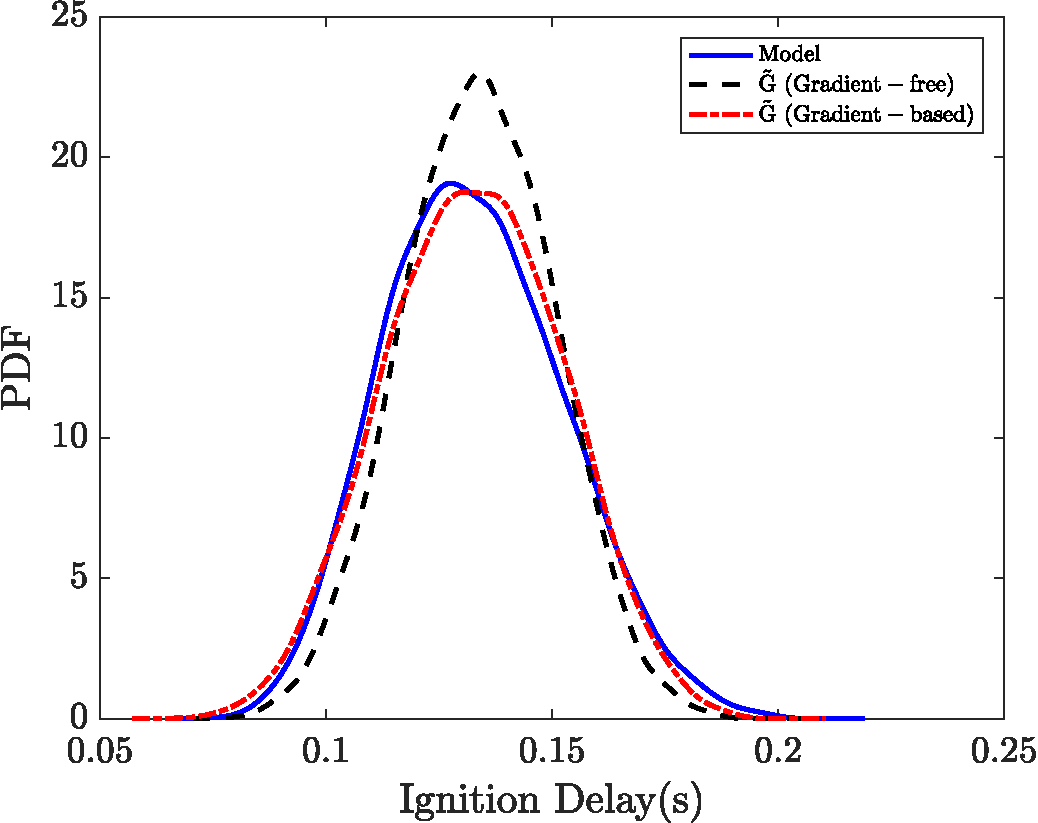
\includegraphics[width=0.45\textwidth]{./Figures/pdf_comp_id_1e4}</span></td>
      </tr>
      <tr>
        <td id="L116" class="blob-num js-line-number" data-line-number="116"></td>
        <td id="LC116" class="blob-code blob-code-inner js-file-line"><span class="pl-c"><span class="pl-c">%</span>\caption{A comparison of the PDFs of ignition delay, obtained using model evaluations (solid line) and</span></td>
      </tr>
      <tr>
        <td id="L117" class="blob-num js-line-number" data-line-number="117"></td>
        <td id="LC117" class="blob-code blob-code-inner js-file-line"><span class="pl-c"><span class="pl-c">%</span>1-dimensional surrogates using the gradient-free approach (dashed line) and the gradient-based approach</span></td>
      </tr>
      <tr>
        <td id="L118" class="blob-num js-line-number" data-line-number="118"></td>
        <td id="LC118" class="blob-code blob-code-inner js-file-line"><span class="pl-c"><span class="pl-c">%</span>(dashed-dotted line). The same set of 10$^4$ samples in the cross-validation set were used in each case.}</span></td>
      </tr>
      <tr>
        <td id="L119" class="blob-num js-line-number" data-line-number="119"></td>
        <td id="LC119" class="blob-code blob-code-inner js-file-line"><span class="pl-c"><span class="pl-c">%</span>\label{fig:pdf_33D}</span></td>
      </tr>
      <tr>
        <td id="L120" class="blob-num js-line-number" data-line-number="120"></td>
        <td id="LC120" class="blob-code blob-code-inner js-file-line"><span class="pl-c"><span class="pl-c">%</span>\end{center}</span></td>
      </tr>
      <tr>
        <td id="L121" class="blob-num js-line-number" data-line-number="121"></td>
        <td id="LC121" class="blob-code blob-code-inner js-file-line"><span class="pl-c"><span class="pl-c">%</span>\end{figure}</span></td>
      </tr>
      <tr>
        <td id="L122" class="blob-num js-line-number" data-line-number="122"></td>
        <td id="LC122" class="blob-code blob-code-inner js-file-line"><span class="pl-c"><span class="pl-c">%</span></span></td>
      </tr>
      <tr>
        <td id="L123" class="blob-num js-line-number" data-line-number="123"></td>
        <td id="LC123" class="blob-code blob-code-inner js-file-line">The PDFs based on the model evaluations and the gradient-based approach are nearly identical, confirming</td>
      </tr>
      <tr>
        <td id="L124" class="blob-num js-line-number" data-line-number="124"></td>
        <td id="LC124" class="blob-code blob-code-inner js-file-line">the existence of a 1-dimensional active subspace as well as the accuracy of the gradient-based approach. </td>
      </tr>
      <tr>
        <td id="L125" class="blob-num js-line-number" data-line-number="125"></td>
        <td id="LC125" class="blob-code blob-code-inner js-file-line">Whereas, the PDF based on the gradient-free approach is observed to show consistency with the true PDF in the modal</td>
      </tr>
      <tr>
        <td id="L126" class="blob-num js-line-number" data-line-number="126"></td>
        <td id="LC126" class="blob-code blob-code-inner js-file-line">estimate; it underestimates the spread in the ignition delay. Specific values of the mean and the standard deviation</td>
      </tr>
      <tr>
        <td id="L127" class="blob-num js-line-number" data-line-number="127"></td>
        <td id="LC127" class="blob-code blob-code-inner js-file-line">in each case are provided in the table in Figure~<span class="pl-c1">\ref</span>{fig:pdf_33D}. Hence, the three PDFs are found to be</td>
      </tr>
      <tr>
        <td id="L128" class="blob-num js-line-number" data-line-number="128"></td>
        <td id="LC128" class="blob-code blob-code-inner js-file-line">consistent in their prediction of mean value of the ignition delay.  The standard deviation estimates based on model</td>
      </tr>
      <tr>
        <td id="L129" class="blob-num js-line-number" data-line-number="129"></td>
        <td id="LC129" class="blob-code blob-code-inner js-file-line">evaluations and the gradient-based approach are found to be in close agreement, whereas, it  is accurately estimated</td>
      </tr>
      <tr>
        <td id="L130" class="blob-num js-line-number" data-line-number="130"></td>
        <td id="LC130" class="blob-code blob-code-inner js-file-line">by the gradient-free approach only upto the first significant figure. </td>
      </tr>
      <tr>
        <td id="L131" class="blob-num js-line-number" data-line-number="131"></td>
        <td id="LC131" class="blob-code blob-code-inner js-file-line">
</td>
      </tr>
      <tr>
        <td id="L132" class="blob-num js-line-number" data-line-number="132"></td>
        <td id="LC132" class="blob-code blob-code-inner js-file-line"><span class="pl-c1">\subsection</span>{GSA consistency check}</td>
      </tr>
      <tr>
        <td id="L133" class="blob-num js-line-number" data-line-number="133"></td>
        <td id="LC133" class="blob-code blob-code-inner js-file-line">
</td>
      </tr>
      <tr>
        <td id="L134" class="blob-num js-line-number" data-line-number="134"></td>
        <td id="LC134" class="blob-code blob-code-inner js-file-line">The normalized activity scores (<span class="pl-s"><span class="pl-pds">$</span><span class="pl-c1">\tilde</span>{<span class="pl-c1">\nu</span>}_{i,r}<span class="pl-pds">$</span></span>) based on the dominant eigenspace using the two</td>
      </tr>
      <tr>
        <td id="L135" class="blob-num js-line-number" data-line-number="135"></td>
        <td id="LC135" class="blob-code blob-code-inner js-file-line">approaches (gradient-based and gradient-free) are compared with the total Sobol&#39; indices</td>
      </tr>
      <tr>
        <td id="L136" class="blob-num js-line-number" data-line-number="136"></td>
        <td id="LC136" class="blob-code blob-code-inner js-file-line">in Figure~<span class="pl-c1">\ref</span>{fig:as_33D}. Note that the Sobol&#39; indices were computed using the verified</td>
      </tr>
      <tr>
        <td id="L137" class="blob-num js-line-number" data-line-number="137"></td>
        <td id="LC137" class="blob-code blob-code-inner js-file-line">1-dimensional surrogate in the active subspace for the gradient-based approach. </td>
      </tr>
      <tr>
        <td id="L138" class="blob-num js-line-number" data-line-number="138"></td>
        <td id="LC138" class="blob-code blob-code-inner js-file-line"><span class="pl-c"><span class="pl-c">%</span></span></td>
      </tr>
      <tr>
        <td id="L139" class="blob-num js-line-number" data-line-number="139"></td>
        <td id="LC139" class="blob-code blob-code-inner js-file-line"><span class="pl-c1">\begin</span>{figure}[htbp]</td>
      </tr>
      <tr>
        <td id="L140" class="blob-num js-line-number" data-line-number="140"></td>
        <td id="LC140" class="blob-code blob-code-inner js-file-line"> <span class="pl-c1">\begin</span>{center}</td>
      </tr>
      <tr>
        <td id="L141" class="blob-num js-line-number" data-line-number="141"></td>
        <td id="LC141" class="blob-code blob-code-inner js-file-line">  <span class="pl-c1">\includegraphics</span>[width=0.8<span class="pl-c1">\textwidth</span>]{./Figures/as_33D_new}</td>
      </tr>
      <tr>
        <td id="L142" class="blob-num js-line-number" data-line-number="142"></td>
        <td id="LC142" class="blob-code blob-code-inner js-file-line"><span class="pl-c1">\caption</span>{A bar-graph illustrating individual activity scores for the uncertain <span class="pl-s"><span class="pl-pds">$</span>A_i<span class="pl-pds">$</span></span>&#39; (left) and <span class="pl-s"><span class="pl-pds">$</span>E_{a,i}<span class="pl-pds">$</span></span>&#39;s (right).}</td>
      </tr>
      <tr>
        <td id="L143" class="blob-num js-line-number" data-line-number="143"></td>
        <td id="LC143" class="blob-code blob-code-inner js-file-line"><span class="pl-c1">\label</span>{fig:as_33D}</td>
      </tr>
      <tr>
        <td id="L144" class="blob-num js-line-number" data-line-number="144"></td>
        <td id="LC144" class="blob-code blob-code-inner js-file-line"><span class="pl-c1">\end</span>{center}</td>
      </tr>
      <tr>
        <td id="L145" class="blob-num js-line-number" data-line-number="145"></td>
        <td id="LC145" class="blob-code blob-code-inner js-file-line"><span class="pl-c1">\end</span>{figure}</td>
      </tr>
      <tr>
        <td id="L146" class="blob-num js-line-number" data-line-number="146"></td>
        <td id="LC146" class="blob-code blob-code-inner js-file-line"><span class="pl-c"><span class="pl-c">%</span></span></td>
      </tr>
      <tr>
        <td id="L147" class="blob-num js-line-number" data-line-number="147"></td>
        <td id="LC147" class="blob-code blob-code-inner js-file-line">Several useful inferences can be drawn from the above plot. Firstly, the total Sobol indices are found to be</td>
      </tr>
      <tr>
        <td id="L148" class="blob-num js-line-number" data-line-number="148"></td>
        <td id="LC148" class="blob-code blob-code-inner js-file-line">consistent</td>
      </tr>
      <tr>
        <td id="L149" class="blob-num js-line-number" data-line-number="149"></td>
        <td id="LC149" class="blob-code blob-code-inner js-file-line">with the normalized activity scores evaluated using the gradient-based approach. Whereas, the gradient-free</td>
      </tr>
      <tr>
        <td id="L150" class="blob-num js-line-number" data-line-number="150"></td>
        <td id="LC150" class="blob-code blob-code-inner js-file-line">approach yields consistent results for the <span class="pl-s"><span class="pl-pds">$</span>A_i<span class="pl-pds">$</span></span>&#39;s, it does not capture the sensitivity associated with</td>
      </tr>
      <tr>
        <td id="L151" class="blob-num js-line-number" data-line-number="151"></td>
        <td id="LC151" class="blob-code blob-code-inner js-file-line"><span class="pl-s"><span class="pl-pds">$</span>E_{a,15}<span class="pl-pds">$</span></span>. While this observation bolsters our confidence in the gradient-based approach, it clearly</td>
      </tr>
      <tr>
        <td id="L152" class="blob-num js-line-number" data-line-number="152"></td>
        <td id="LC152" class="blob-code blob-code-inner js-file-line">underscores the shortcoming of the gradient-free approach. Numerical errors are incurred when approximating</td>
      </tr>
      <tr>
        <td id="L153" class="blob-num js-line-number" data-line-number="153"></td>
        <td id="LC153" class="blob-code blob-code-inner js-file-line">the model gradients using the local linear approximation in this case. </td>
      </tr>
      <tr>
        <td id="L154" class="blob-num js-line-number" data-line-number="154"></td>
        <td id="LC154" class="blob-code blob-code-inner js-file-line">Secondly, our findings indicate that   </td>
      </tr>
      <tr>
        <td id="L155" class="blob-num js-line-number" data-line-number="155"></td>
        <td id="LC155" class="blob-code blob-code-inner js-file-line">the ignition delay is predominantly sensitive towards <span class="pl-s"><span class="pl-pds">$</span>A_<span class="pl-c1">1</span><span class="pl-pds">$</span></span>, <span class="pl-s"><span class="pl-pds">$</span>A_<span class="pl-c1">9</span><span class="pl-pds">$</span></span>, <span class="pl-s"><span class="pl-pds">$</span>E_{a,1}<span class="pl-pds">$</span></span>, and <span class="pl-s"><span class="pl-pds">$</span>E_{a,15}<span class="pl-pds">$</span></span> and </td>
      </tr>
      <tr>
        <td id="L156" class="blob-num js-line-number" data-line-number="156"></td>
        <td id="LC156" class="blob-code blob-code-inner js-file-line">moderately sensitive towards <span class="pl-s"><span class="pl-pds">$</span>A_{15}<span class="pl-pds">$</span></span> and <span class="pl-s"><span class="pl-pds">$</span>A_{17}<span class="pl-pds">$</span></span>. Sensitivity towards the remaining uncertain inputs is</td>
      </tr>
      <tr>
        <td id="L157" class="blob-num js-line-number" data-line-number="157"></td>
        <td id="LC157" class="blob-code blob-code-inner js-file-line">found to be low or negligible. </td>
      </tr>
      <tr>
        <td id="L158" class="blob-num js-line-number" data-line-number="158"></td>
        <td id="LC158" class="blob-code blob-code-inner js-file-line"><span class="pl-c"><span class="pl-c">%</span>Note that this observation can also be exploited for reducing the </span></td>
      </tr>
      <tr>
        <td id="L159" class="blob-num js-line-number" data-line-number="159"></td>
        <td id="LC159" class="blob-code blob-code-inner js-file-line"><span class="pl-c"><span class="pl-c">%</span>dimensionality of the problem from 33 inputs to 4-6 inputs depending upon the required level of accuracy.</span></td>
      </tr>
      <tr>
        <td id="L160" class="blob-num js-line-number" data-line-number="160"></td>
        <td id="LC160" class="blob-code blob-code-inner js-file-line"><span class="pl-c"><span class="pl-c">%</span>The sensitivity-driven dimension reduction for uncertainty quantification has been</span></td>
      </tr>
      <tr>
        <td id="L161" class="blob-num js-line-number" data-line-number="161"></td>
        <td id="LC161" class="blob-code blob-code-inner js-file-line"><span class="pl-c"><span class="pl-c">%</span>discussed in our earlier effort~\cite{Vohra:2018}. In this work, however, we focus on dimension reduction using the active </span></td>
      </tr>
      <tr>
        <td id="L162" class="blob-num js-line-number" data-line-number="162"></td>
        <td id="LC162" class="blob-code blob-code-inner js-file-line"><span class="pl-c"><span class="pl-c">%</span>subspace approach which is shown to yield even greater scope for dimension reduction i.e. from 33 to 1. Furthermore, we have</span></td>
      </tr>
      <tr>
        <td id="L163" class="blob-num js-line-number" data-line-number="163"></td>
        <td id="LC163" class="blob-code blob-code-inner js-file-line"><span class="pl-c"><span class="pl-c">%</span>shown that the dominant eigenspace can be used to approximate global sensitivity measures with no additional effort.</span></td>
      </tr>
      <tr>
        <td id="L164" class="blob-num js-line-number" data-line-number="164"></td>
        <td id="LC164" class="blob-code blob-code-inner js-file-line">
</td>
      </tr>
      <tr>
        <td id="L165" class="blob-num js-line-number" data-line-number="165"></td>
        <td id="LC165" class="blob-code blob-code-inner js-file-line">
</td>
      </tr>
      <tr>
        <td id="L166" class="blob-num js-line-number" data-line-number="166"></td>
        <td id="LC166" class="blob-code blob-code-inner js-file-line">
</td>
      </tr>
      <tr>
        <td id="L167" class="blob-num js-line-number" data-line-number="167"></td>
        <td id="LC167" class="blob-code blob-code-inner js-file-line">
</td>
      </tr>
      <tr>
        <td id="L168" class="blob-num js-line-number" data-line-number="168"></td>
        <td id="LC168" class="blob-code blob-code-inner js-file-line">
</td>
      </tr>
      <tr>
        <td id="L169" class="blob-num js-line-number" data-line-number="169"></td>
        <td id="LC169" class="blob-code blob-code-inner js-file-line">
</td>
      </tr>
      <tr>
        <td id="L170" class="blob-num js-line-number" data-line-number="170"></td>
        <td id="LC170" class="blob-code blob-code-inner js-file-line">
</td>
      </tr>
      <tr>
        <td id="L171" class="blob-num js-line-number" data-line-number="171"></td>
        <td id="LC171" class="blob-code blob-code-inner js-file-line">
</td>
      </tr>
      <tr>
        <td id="L172" class="blob-num js-line-number" data-line-number="172"></td>
        <td id="LC172" class="blob-code blob-code-inner js-file-line">
</td>
      </tr>
      <tr>
        <td id="L173" class="blob-num js-line-number" data-line-number="173"></td>
        <td id="LC173" class="blob-code blob-code-inner js-file-line">
</td>
      </tr>
      <tr>
        <td id="L174" class="blob-num js-line-number" data-line-number="174"></td>
        <td id="LC174" class="blob-code blob-code-inner js-file-line">
</td>
      </tr>
      <tr>
        <td id="L175" class="blob-num js-line-number" data-line-number="175"></td>
        <td id="LC175" class="blob-code blob-code-inner js-file-line">
</td>
      </tr>
      <tr>
        <td id="L176" class="blob-num js-line-number" data-line-number="176"></td>
        <td id="LC176" class="blob-code blob-code-inner js-file-line">
</td>
      </tr>
      <tr>
        <td id="L177" class="blob-num js-line-number" data-line-number="177"></td>
        <td id="LC177" class="blob-code blob-code-inner js-file-line">
</td>
      </tr>
      <tr>
        <td id="L178" class="blob-num js-line-number" data-line-number="178"></td>
        <td id="LC178" class="blob-code blob-code-inner js-file-line">
</td>
      </tr>
      <tr>
        <td id="L179" class="blob-num js-line-number" data-line-number="179"></td>
        <td id="LC179" class="blob-code blob-code-inner js-file-line">
</td>
      </tr>
      <tr>
        <td id="L180" class="blob-num js-line-number" data-line-number="180"></td>
        <td id="LC180" class="blob-code blob-code-inner js-file-line">
</td>
      </tr>
      <tr>
        <td id="L181" class="blob-num js-line-number" data-line-number="181"></td>
        <td id="LC181" class="blob-code blob-code-inner js-file-line">
</td>
      </tr>
      <tr>
        <td id="L182" class="blob-num js-line-number" data-line-number="182"></td>
        <td id="LC182" class="blob-code blob-code-inner js-file-line">
</td>
      </tr>
      <tr>
        <td id="L183" class="blob-num js-line-number" data-line-number="183"></td>
        <td id="LC183" class="blob-code blob-code-inner js-file-line">
</td>
      </tr>
      <tr>
        <td id="L184" class="blob-num js-line-number" data-line-number="184"></td>
        <td id="LC184" class="blob-code blob-code-inner js-file-line">
</td>
      </tr>
      <tr>
        <td id="L185" class="blob-num js-line-number" data-line-number="185"></td>
        <td id="LC185" class="blob-code blob-code-inner js-file-line">
</td>
      </tr>
      <tr>
        <td id="L186" class="blob-num js-line-number" data-line-number="186"></td>
        <td id="LC186" class="blob-code blob-code-inner js-file-line">
</td>
      </tr>
      <tr>
        <td id="L187" class="blob-num js-line-number" data-line-number="187"></td>
        <td id="LC187" class="blob-code blob-code-inner js-file-line">
</td>
      </tr>
      <tr>
        <td id="L188" class="blob-num js-line-number" data-line-number="188"></td>
        <td id="LC188" class="blob-code blob-code-inner js-file-line">
</td>
      </tr>
      <tr>
        <td id="L189" class="blob-num js-line-number" data-line-number="189"></td>
        <td id="LC189" class="blob-code blob-code-inner js-file-line">
</td>
      </tr>
      <tr>
        <td id="L190" class="blob-num js-line-number" data-line-number="190"></td>
        <td id="LC190" class="blob-code blob-code-inner js-file-line">
</td>
      </tr>
      <tr>
        <td id="L191" class="blob-num js-line-number" data-line-number="191"></td>
        <td id="LC191" class="blob-code blob-code-inner js-file-line">
</td>
      </tr>
      <tr>
        <td id="L192" class="blob-num js-line-number" data-line-number="192"></td>
        <td id="LC192" class="blob-code blob-code-inner js-file-line">
</td>
      </tr>
      <tr>
        <td id="L193" class="blob-num js-line-number" data-line-number="193"></td>
        <td id="LC193" class="blob-code blob-code-inner js-file-line">
</td>
      </tr>
      <tr>
        <td id="L194" class="blob-num js-line-number" data-line-number="194"></td>
        <td id="LC194" class="blob-code blob-code-inner js-file-line">
</td>
      </tr>
      <tr>
        <td id="L195" class="blob-num js-line-number" data-line-number="195"></td>
        <td id="LC195" class="blob-code blob-code-inner js-file-line">
</td>
      </tr>
</table>

  <details class="details-reset details-overlay BlobToolbar position-absolute js-file-line-actions dropdown d-none" aria-hidden="true">
    <summary class="btn-octicon ml-0 px-2 p-0 bg-white border border-gray-dark rounded-1" aria-label="Inline file action toolbar">
      <svg class="octicon octicon-kebab-horizontal" viewBox="0 0 13 16" version="1.1" width="13" height="16" aria-hidden="true"><path fill-rule="evenodd" d="M1.5 9a1.5 1.5 0 1 0 0-3 1.5 1.5 0 0 0 0 3zm5 0a1.5 1.5 0 1 0 0-3 1.5 1.5 0 0 0 0 3zM13 7.5a1.5 1.5 0 1 1-3 0 1.5 1.5 0 0 1 3 0z"/></svg>
    </summary>
    <details-menu>
      <ul class="BlobToolbar-dropdown dropdown-menu dropdown-menu-se mt-2">
        <li><clipboard-copy role="menuitem" class="dropdown-item" id="js-copy-lines" style="cursor:pointer;" data-original-text="Copy lines">Copy lines</clipboard-copy></li>
        <li><clipboard-copy role="menuitem" class="dropdown-item" id="js-copy-permalink" style="cursor:pointer;" data-original-text="Copy permalink">Copy permalink</clipboard-copy></li>
        <li><a class="dropdown-item js-update-url-with-hash" id="js-view-git-blame" role="menuitem" href="/vohramanav/ActiveSubspace_Kinetics/blame/de781a8c95a3c79c7d21d73d7c02fb74af163b10/Paper/app.tex">View git blame</a></li>
          <li><a class="dropdown-item" id="js-new-issue" role="menuitem" href="/vohramanav/ActiveSubspace_Kinetics/issues/new">Open new issue</a></li>
      </ul>
    </details-menu>
  </details>

  </div>

  </div>

  <details class="details-reset details-overlay details-overlay-dark">
    <summary data-hotkey="l" aria-label="Jump to line"></summary>
    <details-dialog class="Box Box--overlay d-flex flex-column anim-fade-in fast linejump" aria-label="Jump to line">
      <!-- '"` --><!-- </textarea></xmp> --></option></form><form class="js-jump-to-line-form Box-body d-flex" action="" accept-charset="UTF-8" method="get"><input name="utf8" type="hidden" value="&#x2713;" />
        <input class="form-control flex-auto mr-3 linejump-input js-jump-to-line-field" type="text" placeholder="Jump to line&hellip;" aria-label="Jump to line" autofocus>
        <button type="submit" class="btn" data-close-dialog>Go</button>
</form>    </details-dialog>
  </details>


  </div>
  <div class="modal-backdrop js-touch-events"></div>
</div>

    </div>
  </div>

  </div>

        
<div class="footer container-lg px-3" role="contentinfo">
  <div class="position-relative d-flex flex-justify-between pt-6 pb-2 mt-6 f6 text-gray border-top border-gray-light ">
    <ul class="list-style-none d-flex flex-wrap ">
      <li class="mr-3">&copy; 2018 <span title="0.29776s from unicorn-5d658c9fd8-qzbnt">GitHub</span>, Inc.</li>
        <li class="mr-3"><a data-ga-click="Footer, go to terms, text:terms" href="https://github.com/site/terms">Terms</a></li>
        <li class="mr-3"><a data-ga-click="Footer, go to privacy, text:privacy" href="https://github.com/site/privacy">Privacy</a></li>
        <li class="mr-3"><a href="https://help.github.com/articles/github-security/" data-ga-click="Footer, go to security, text:security">Security</a></li>
        <li class="mr-3"><a href="https://status.github.com/" data-ga-click="Footer, go to status, text:status">Status</a></li>
        <li><a data-ga-click="Footer, go to help, text:help" href="https://help.github.com">Help</a></li>
    </ul>

    <a aria-label="Homepage" title="GitHub" class="footer-octicon" href="https://github.com">
      <svg height="24" class="octicon octicon-mark-github" viewBox="0 0 16 16" version="1.1" width="24" aria-hidden="true"><path fill-rule="evenodd" d="M8 0C3.58 0 0 3.58 0 8c0 3.54 2.29 6.53 5.47 7.59.4.07.55-.17.55-.38 0-.19-.01-.82-.01-1.49-2.01.37-2.53-.49-2.69-.94-.09-.23-.48-.94-.82-1.13-.28-.15-.68-.52-.01-.53.63-.01 1.08.58 1.23.82.72 1.21 1.87.87 2.33.66.07-.52.28-.87.51-1.07-1.78-.2-3.64-.89-3.64-3.95 0-.87.31-1.59.82-2.15-.08-.2-.36-1.02.08-2.12 0 0 .67-.21 2.2.82.64-.18 1.32-.27 2-.27.68 0 1.36.09 2 .27 1.53-1.04 2.2-.82 2.2-.82.44 1.1.16 1.92.08 2.12.51.56.82 1.27.82 2.15 0 3.07-1.87 3.75-3.65 3.95.29.25.54.73.54 1.48 0 1.07-.01 1.93-.01 2.2 0 .21.15.46.55.38A8.013 8.013 0 0 0 16 8c0-4.42-3.58-8-8-8z"/></svg>
</a>
   <ul class="list-style-none d-flex flex-wrap ">
        <li class="mr-3"><a data-ga-click="Footer, go to contact, text:contact" href="https://github.com/contact">Contact GitHub</a></li>
        <li class="mr-3"><a href="https://github.com/pricing" data-ga-click="Footer, go to Pricing, text:Pricing">Pricing</a></li>
      <li class="mr-3"><a href="https://developer.github.com" data-ga-click="Footer, go to api, text:api">API</a></li>
      <li class="mr-3"><a href="https://training.github.com" data-ga-click="Footer, go to training, text:training">Training</a></li>
        <li class="mr-3"><a href="https://blog.github.com" data-ga-click="Footer, go to blog, text:blog">Blog</a></li>
        <li><a data-ga-click="Footer, go to about, text:about" href="https://github.com/about">About</a></li>

    </ul>
  </div>
  <div class="d-flex flex-justify-center pb-6">
    <span class="f6 text-gray-light"></span>
  </div>
</div>



  <div id="ajax-error-message" class="ajax-error-message flash flash-error">
    <svg class="octicon octicon-alert" viewBox="0 0 16 16" version="1.1" width="16" height="16" aria-hidden="true"><path fill-rule="evenodd" d="M8.893 1.5c-.183-.31-.52-.5-.887-.5s-.703.19-.886.5L.138 13.499a.98.98 0 0 0 0 1.001c.193.31.53.501.886.501h13.964c.367 0 .704-.19.877-.5a1.03 1.03 0 0 0 .01-1.002L8.893 1.5zm.133 11.497H6.987v-2.003h2.039v2.003zm0-3.004H6.987V5.987h2.039v4.006z"/></svg>
    <button type="button" class="flash-close js-ajax-error-dismiss" aria-label="Dismiss error">
      <svg class="octicon octicon-x" viewBox="0 0 12 16" version="1.1" width="12" height="16" aria-hidden="true"><path fill-rule="evenodd" d="M7.48 8l3.75 3.75-1.48 1.48L6 9.48l-3.75 3.75-1.48-1.48L4.52 8 .77 4.25l1.48-1.48L6 6.52l3.75-3.75 1.48 1.48L7.48 8z"/></svg>
    </button>
    You can’t perform that action at this time.
  </div>


    <script crossorigin="anonymous" integrity="sha512-2VdGgXQE8W5ONZ4OsrbEo/noennUZaqXkevD9R8juTHiCsjT0HFTTF6MoBfySUc8G+eFqUcDgd7v+CAu8Gjxlg==" type="application/javascript" src="https://assets-cdn.github.com/assets/compat-f849c975b0ffaa01d6ca305e48417d08.js"></script>
    <script crossorigin="anonymous" integrity="sha512-xY0/FVA4OIId4Rg/UZwnuRt3NDzYfohwWB8mPrflYnyu+RSIdK8VxsCY3VkctCpeCW5BSB331jAUlVEbupUlGQ==" type="application/javascript" src="https://assets-cdn.github.com/assets/frameworks-caa0bdcb0cd0270ade93e4f0358e158e.js"></script>
    
    <script crossorigin="anonymous" async="async" integrity="sha512-/gomoh+vz4Wtp3+45P6w1H96O3k/a09vbwD6g3etmqocBu12fflwXz0oFmWYELM1Kh85wnXuBytcmGv4QSca6w==" type="application/javascript" src="https://assets-cdn.github.com/assets/github-69f027cf810a992224f91b6f505ea246.js"></script>
    
    
    
  <div class="js-stale-session-flash stale-session-flash flash flash-warn flash-banner d-none">
    <svg class="octicon octicon-alert" viewBox="0 0 16 16" version="1.1" width="16" height="16" aria-hidden="true"><path fill-rule="evenodd" d="M8.893 1.5c-.183-.31-.52-.5-.887-.5s-.703.19-.886.5L.138 13.499a.98.98 0 0 0 0 1.001c.193.31.53.501.886.501h13.964c.367 0 .704-.19.877-.5a1.03 1.03 0 0 0 .01-1.002L8.893 1.5zm.133 11.497H6.987v-2.003h2.039v2.003zm0-3.004H6.987V5.987h2.039v4.006z"/></svg>
    <span class="signed-in-tab-flash">You signed in with another tab or window. <a href="">Reload</a> to refresh your session.</span>
    <span class="signed-out-tab-flash">You signed out in another tab or window. <a href="">Reload</a> to refresh your session.</span>
  </div>
  <div class="facebox" id="facebox" style="display:none;">
  <div class="facebox-popup">
    <div class="facebox-content" role="dialog" aria-labelledby="facebox-header" aria-describedby="facebox-description">
    </div>
    <button type="button" class="facebox-close js-facebox-close" aria-label="Close modal">
      <svg class="octicon octicon-x" viewBox="0 0 12 16" version="1.1" width="12" height="16" aria-hidden="true"><path fill-rule="evenodd" d="M7.48 8l3.75 3.75-1.48 1.48L6 9.48l-3.75 3.75-1.48-1.48L4.52 8 .77 4.25l1.48-1.48L6 6.52l3.75-3.75 1.48 1.48L7.48 8z"/></svg>
    </button>
  </div>
</div>

  <template id="site-details-dialog">
  <details class="details-reset details-overlay details-overlay-dark lh-default text-gray-dark" open>
    <summary aria-haspopup="dialog" aria-label="Close dialog"></summary>
    <details-dialog class="Box Box--overlay d-flex flex-column anim-fade-in fast">
      <button class="m-3 btn-octicon position-absolute right-0 top-0" type="button" aria-label="Close dialog" data-close-dialog>
        <svg class="octicon octicon-x" viewBox="0 0 12 16" version="1.1" width="12" height="16" aria-hidden="true"><path fill-rule="evenodd" d="M7.48 8l3.75 3.75-1.48 1.48L6 9.48l-3.75 3.75-1.48-1.48L4.52 8 .77 4.25l1.48-1.48L6 6.52l3.75-3.75 1.48 1.48L7.48 8z"/></svg>
      </button>
      <div class="octocat-spinner my-6 js-details-dialog-spinner"></div>
    </details-dialog>
  </details>
</template>

  <div class="Popover js-hovercard-content position-absolute" style="display: none; outline: none;" tabindex="0">
  <div class="Popover-message Popover-message--bottom-left Popover-message--large Box box-shadow-large" style="width:360px;">
  </div>
</div>

<div id="hovercard-aria-description" class="sr-only">
  Press h to open a hovercard with more details.
</div>


  </body>
</html>

